\documentclass[10pt]{article}
\usepackage{amsmath,amssymb,graphicx,booktabs,geometry}
\usepackage{multirow}
\usepackage{float}
\usepackage{caption}
\usepackage{subcaption}
\usepackage{enumitem}
\usepackage{hyperref}
\geometry{margin=1in}
\captionsetup{font=small,labelfont=bf}
\setlength{\textfloatsep}{6pt plus 2pt minus 2pt}
\setlength{\floatsep}{6pt plus 2pt minus 2pt}
\setlength{\dbltextfloatsep}{6pt}
\setlength{\intextsep}{10pt plus 2pt minus 2pt}
\setlength{\abovecaptionskip}{6pt}
\setlength{\belowcaptionskip}{2pt}

\title{Recovering the Hidden Ballot: A Survival--Belief Inversion of Latent Fan Votes, \\
a Replay Engine for Rank vs.\ Percentage Combination Rules, and a \\
Two-Channel Covariate Analysis of 34 Seasons of \textit{Dancing with the Stars}}

\author{Team 2481 --- 2026 MCM Problem C}
\date{January 2026}

\begin{document}
\maketitle
\tableofcontents
\newpage

\begin{abstract}
\textit{Dancing with the Stars} combines expert judge scores with audience fan votes to
decide each week's elimination, yet the fan votes themselves are never released. We
reconstruct them. Using 34 seasons of per-judge scores, contestant demographics, and the
elimination record (2{,}777 celebrity-weeks, 297 elimination events), Model 1 inverts a
discrete-time cloglog elimination hazard fused with a Dempster--Shafer belief layer and
couple-level frailty to produce weekly fan-vote share estimates $\hat\phi_{iw}$ with
honest, contestant- and week-specific 90\% intervals (median width 0.095 share points).
The estimates are strongly consistent with the observed record: the actually eliminated
couple has the lowest estimated share in 67.0\% of elimination events (bottom-two in
89.6\%), simulated elimination probability achieves AUC 0.959 (Brier 0.047; mean
predicted 0.109 vs.\ observed 0.108), and final share tracks final placement at Kendall
$\tau = +0.799$ --- all far above judge-only baselines (42.8\% top-1). Holdout
leave-one-season-out checks confirm stability (AUC drop 0.008). Model 2 then replays all
34 seasons under the show's rank-based and percentage-based combination rules using the
same $\hat\phi$: the era-correct engine reproduces 88.9\% of cuts (100\% in the rank era,
99.2\% in the percentage era), yet the two rules disagree in 48.7\% of elimination weeks
--- including the season-9 championship, where the percentage rule crowns Mya and the
rank rule does not. Controversy verdicts decompose into rule-invariant (Jerry Rice, S2),
method-attributable (Bristol Palin S11, Mya S9), and fan-driven cases that no rule
reproduces (Bobby Bones' S27 win). From season 28, reproduction collapses from 89.2\%
to 50.8\% unless the judges' dance-off stage is modeled --- evidence that the stage, not
the combination rule, drives modern-era divergence. Model 3's two-channel analysis shows
the judges' channel is roughly $2.5\times$ more age-sensitive than the fans' channel
($-0.477$ vs.\ $-0.158$ per centered decade), with several industry effects flipping sign
between channels. We recommend a hybrid system: percentage-based combination (shock rate
0.3\% vs.\ 3.8\%/5.0\%) plus a deterministic top-quartile judge floor and a
finale-only dance-off.
\end{abstract}

\textbf{Keywords:} fan-vote inversion; survival analysis; Dempster--Shafer theory;
counterfactual replay; mixed-effects models; \textit{Dancing with the Stars}.

%=====================================================================
\section{Introduction}
%=====================================================================

\subsection{Problem Background and Motivation}

\textit{Dancing with the Stars} (DWTS), the American adaptation of the British franchise
\textit{Strictly Come Dancing}, has completed 34 seasons. Each season, celebrities are
paired with professional dancers and perform weekly; a panel of expert judges scores each
couple's dance on a 10-point scale, and fans vote for their favorite couple. The judges'
scores and the fans' votes are combined --- and it is precisely the \emph{combination rule}
that determines who survives each week and who is eliminated. Three couples (in some
seasons more, four or five) reach a finale in which the combined score ranks the remaining
field from first to last.

The show's combination machinery has never been static. In seasons 1--2 the producers used
a \emph{rank-based} rule: the couple with the lowest combined rank of judge placement and
fan placement is eliminated. Concerns raised in season 2 by the run of contestant Jerry
Rice --- a finalist despite some of the lowest judge scores of the season --- prompted a
switch to \emph{percentage-based} combination from season 3 onward, in which normalized
judge and fan vote \emph{shares} are added rather than ranks. In season 27 a new
controversy erupted when radio host Bobby Bones won the mirror-ball trophy despite
consistently low judge scores; from season 28 the producers responded both by returning to
rank-based combination (assumed to be season 28, the exact season undocumented) and by
adding a \emph{judges' dance-off} stage in which the bottom-two couples are identified by
the combined score but the judges themselves choose which of the two is eliminated.

Two facts make this system interesting and difficult to model. First, \textbf{fan votes are
secret}. The show never releases per-contestant vote totals, so any quantitative study of
the combination rules --- or of who ``really'' kept a popular but technically weak
contestant alive --- must reconstruct the latent votes from the only observable evidence:
weekly judge scores and the elimination record. Second, the observable evidence is
\emph{partial but informative}: each week the show reveals a bottom-two (or bottom-three)
nomination and one (or more) cut(s), which strongly constrains the lower tail of the
unobserved fan-vote distribution, even though it says little about the ordering of the
upper half of the field.

This report develops three linked mathematical models that convert 34 seasons of public
scores and outcomes into: (i) estimated fan-vote \emph{shares} for every couple in every
week they danced, with honest per-couple, per-week uncertainty; (ii) a counterfactual
replay engine that quantifies how the rank-based versus percentage-based combination rules
change --- or fail to change --- elimination histories, including those of the show's most
famous controversies; and (iii) a two-channel regression analysis of how celebrity
characteristics (age, industry, professional partner) propagate differently into judge
scores and fan support.

\subsection{Data Description}

The provided dataset \texttt{2026\_MCM\_Problem\_C\_Data.csv} contains 421 celebrity-season
rows (one row per celebrity per season; some professionals' celebrity partners recur) and
53 columns: celebrity name, professional partner, celebrity industry, home state, home
country/region, age during the season, season number (1--34), the season-end result string
(e.g.\ ``1st Place''), final placement, and 44 weekly judge-score columns (weeks 1--11
$\times$ judges 1--4, with \texttt{N/A} for absent panels/weeks). Key structural features
discovered during data exploration, and codified in the shared preprocessing layer
(\texttt{prep\_data.py}, with all checks passing):

\begin{itemize}[itemsep=2pt]
\item \textbf{Zeros are filler, not scores.} Raw score cells use 0 where a judge did not
score a dance; \texttt{N/A} marks weeks the couple did not dance. The preprocessing layer
builds \texttt{weekly\_scores.csv} with 2{,}777 celebrity-danced-week rows, keeping only
positive scores and computing the per-dance average judge score $S_{iw}$, the within-week
judge share $\rho_{iw}=S_{iw}/\sum_k S_{kw}$, the within-week judge rank, and the judges'
percentile rank.
\item \textbf{Aggregate scoring weeks.} Later seasons replace per-judge columns with
encoded totals in some weeks; 326 of the 335 season-weeks use redistributed totals. All
models consume only encoding-invariant quantities (share, rank), so mixed encodings are
handled uniformly.
\item \textbf{Panel size varies.} The number of scoring judges ranges from 2 to 4
(mean 3.28); a \texttt{fourth\_judge\_used} flag is carried in \texttt{week\_panel.csv}
(335 season-week rows with competitor counts and elimination counts, allowing double
eliminations such as season 33 weeks 2--3 and season 34 week 2).
\item \textbf{Outcomes.} Each row carries a status (eliminated / withdrew / finalist),
elimination week, and final placement. 39 withdrew contestants are excluded from
elimination supervision; doubles elimination weeks enter the likelihood as multiple
ordered cuts.
\item \textbf{Population summary.} 2{,}777 danced celebrity-weeks across 34 seasons and
408 distinct couples; 297 elimination events (298 eliminated contestants; see the Model 2
quota discussion of the season 18 +1 artifact); 114 censored finalists; active casts range
from 2 (finals) to 16 (largest season-premiere fields), with mean 9.5 active couples per
week.
\item \textbf{Ages span 14--82} (mean 36.3), and the industry field contains 19 distinct
labels from Actor/Actress (882 danced-weeks) and Athlete (616) to Astronaut (3).
\end{itemize}

No external data were used; all covariates come from the provided file. Because fan votes
are never released, the dataset also contains \emph{no} direct fan signal --- this absence
is the central modeling challenge, not an oversight.

\subsection{Our Approach in Brief}
\label{sec:modelintro}

The three models form a deliberate pipeline (Table~\ref{tab:deliverablemap}):

\begin{enumerate}[itemsep=2pt]
\item \textbf{Model 1 (Sections~\ref{sec:model1}--\ref{sec:m1res}) --- Sub-seasonal
survival inversion of latent fan votes.} A discrete-time complementary log-log hazard for
bottom-two nomination (with couple-level frailty capturing unexplained fan pressure),
fused with a truncated Dempster--Shafer belief layer built from judge-share evidence,
produces a weekly fan-vote share estimate $\hat\phi_{iw}$ (summing to 1 within each
season-week) with Beta pseudo-ballot 90\% intervals. Validated by Monte-Carlo elimination
simulation: top-1 elimination hit 0.670, top-2 replication 0.896, AUC 0.959, Kendall
$\tau = +0.799$ between final share and placement.
\item \textbf{Model 2 (Sections~\ref{sec:model2}--\ref{sec:m2results}) --- Judge--fan
fusion and counterfactual replay engine.} A single Module-1-compatible estimator
(couple-level fan-appeal $u_i$ fitted by coordinate ascent over a softmax weekly share
model) supplies $\hat\phi$ for an era-correct replay that reproduces the observed record
(88.9\% mean per-season cut-match rate), then replays all 34 seasons under the rank rule
$R$, percentage rule $P$, and z-scored rule $Z$, and dissects eight named controversies
plus a 90\%-band-edge sensitivity pass.
\item \textbf{Model 3 (Sections~\ref{sec:model3}--\ref{sec:m3valid}) --- Celebrity-covariate
impact model.} Four deliveries: (D1) a mixed-effects model of weekly judge scores;
(D2) a weighted binomial GEE for the fan channel using Model 1's $\hat\phi$ (uncertainty
propagated via $1/\mathrm{Var}$ weights); (D3) an OLS differential model on
$z(S) - z(\hat\phi)$ identifying traits where fans and judges disagree; and (D4) Cox
survival models quantifying how much trait effects are mediated by the two score channels.
\end{enumerate}

\begin{table}[H]
\centering
\caption{Pipeline schematic and deliverable map. The shared preprocessing layer
(\texttt{prep\_data.py}, all checks passing) produces three tables ---
\texttt{contestants.csv} (421 rows), \texttt{weekly\_scores.csv} (2{,}777 danced
celebrity-weeks), and \texttt{week\_panel.csv} (335 season-weeks). Model 1 consumes
the judge scores plus the elimination record and produces the single shared latent
quantity $\hat\phi$ with its uncertainty bands; Models 2 and 3 consume $\hat\phi$
\emph{without refitting it}, guaranteeing one consistent latent-vote story throughout
the report.}
\label{tab:deliverablemap}
\begin{tabular}{p{2.6cm}p{5.4cm}p{5.6cm}}
\toprule
Model & Core quantity & Contest question answered \\
\midrule
Model 1 (Sec.~\ref{sec:model1}) & $\hat\phi_{iw}$: weekly fan-vote share + 90\% bands
& Q1: estimate fan votes; consistency with eliminations; certainty \\
Model 2 (Sec.~\ref{sec:model2}) & counterfactual elimination replays under rules $R$, $P$, $Z$
& Q2: rank vs.\ percentage; controversies; judges' dance-off \\
Model 3 (Sec.~\ref{sec:model3}) & trait effects on judge vs.\ fan channels + survival
& Q3: do age/industry/partner move judges and fans differently \\
\bottomrule
\end{tabular}
\end{table}

\textbf{A note on the two fan-vote estimators.} Two independently implemented inversion
layers appear in this work: Model 1's survival--belief fusion (the fully instrumented
estimator, with belief intervals, calibration, and DSM analysis) and Model 2's
Module-1-compatible softmax estimator (built because no upstream fan-vote table existed at
implementation time). They are calibrated to the same constraints ($\hat\phi$ sums to 1 per
season-week, same 2{,}777--2{,}780 danced-week rows) and produce qualitatively identical
stories for every controversy examined; where their numbers differ the paper reports which
estimator the figure or table comes from. This is consciously \emph{not} presented as two
independent confirmations of the same phenomenon --- they share data, structure, and some
validation logic.

\subsection{Paper Outline}

Section~\ref{sec:model1} formulates and validates Model 1. Section~\ref{sec:model2}
formulates and validates Model 2 and reports the rank-versus-percentage replay and
controversy analysis. Section~\ref{sec:model3} formulates and validates Model 3 and
reports the covariate-impact findings. Section~\ref{sec:results} integrates results across
models and answers each contest question directly; Section~\ref{sec:sensitivity} reports
sensitivity analyses; Section~\ref{sec:discussion} discusses strengths, limitations, and
the proposed alternative scoring system; Section~\ref{sec:conclusion} concludes with
recommendations for the producers.

%=====================================================================
\section{Model 1: Sub-Seasonal Survival Inversion of Latent Fan Votes}
\label{sec:model1}

\subsection{Problem Statement}

The quantity the contest asks us to estimate --- per-couple weekly fan vote totals ---
is never observed. What \emph{is} observed, each week, is (a) every couple's judge score
and (b) which couple (or couples) was eliminated, following a combination of judge scores
with the (hidden) fan votes. The lowest combined score is the eliminated couple, hence the
elimination event is evidence of a \emph{tail event} in the joint distribution of judge
and fan support. Model 1 converts this partial evidence into a Bayesian/belief-function
estimate of the latent fan-vote \emph{share} $\phi_{iw}$ of couple $i$ in week $w$,
together with per-couple, per-week uncertainty bands, and then validates those estimates
against the elimination record by Monte-Carlo simulation.

Three modeling desiderata drive the design:
\begin{enumerate}[itemsep=1pt]
\item \textbf{Consistency:} eliminating the couple with the minimum $\hat\phi$ in each
week should recover the actually eliminated couple substantially more often than a
judge-scores-only baseline.
\item \textbf{Certainty:} the 90\% intervals should be contestant- and week-specific,
wider where the evidence is weak (large casts, contentious weeks) and narrower where it is
strong (small casts, high judge-panel agreement, low frailty variance).
\item \textbf{Sums to one:} within each season-week, $\sum_i \hat\phi_{iw} = 1$ exactly,
since fan votes are shares of a fixed voting pool.
\end{enumerate}

\subsection{Mathematical Formulation}

\subsubsection{The latent-vote model}

For each season $s$ and week $w$, the fan vote is a multinomial over the $n_w$ active
couples:
\begin{equation}
(V_{1w},\dots,V_{n_w w}) \sim \mathrm{Multinomial}(1;\ \phi_{1w},\dots,\phi_{n_w w}),
\qquad \phi_{iw}>0,\quad \sum_{i=1}^{n_w}\phi_{iw}=1.
\label{eq:multinomial}
\end{equation}
We never observe $V$; we observe the elimination event $y_{iw}$ (couple eliminated at end
of week $w$) and, in the S28+ era, the bottom-two nomination.

\subsubsection{Stage A: discrete-time cloglog hazard}

Pre-registration of the model: the weekly \emph{hazard} of bottom-two nomination for
couple $i$ in week $w$ follows a complementary log-log link,
\begin{equation}
\mathrm{cloglog}\,\lambda_{iw} \;=\; \log(-\log \lambda_{iw}) \;=\; \alpha_{w}
+ \beta_1\,\mathrm{judge\_pct}_{iw} + \beta_2\,\mathrm{cum\_pct}_{iw}
+ x_{iw}^{\top}\boldsymbol\gamma + u_i,
\label{eq:hazard}
\end{equation}
where $\alpha_w$ are non-parametric week-stratum baseline hazards (one per week-index
$w=1,\dots,11$, estimated freely, Breslow-type --- no parametric shape is imposed on the
within-season decay of survival as casts shrink), $\mathrm{judge\_pct}_{iw}$ is the
judges' percentile rank of $S_{iw}$ within week $w$, $\mathrm{cum\_pct}_{iw}$ is the
season-normalized cumulative judge percentile, $x_{iw}$ collects industry and partner
covariates, and $u_i$ is a \emph{couple-level frailty} intended to absorb fan pressure not
explained by judges. The survival contribution to the likelihood is the product over the
couple's danced weeks of the hazards until the (observed) elimination week; finalists are
censored at their last danced week. Withdrawn contestants (39 rows) are excluded from
supervision.

\subsubsection{Stage B: Dempster--Shafer belief layer}

Within each season-week, the judges' scores are converted into evidence masses over sets
of couples via a normalized plausibility transform of the within-week share vector:
\begin{equation}
m_j(\{i\}) = \mathrm{softmax}_i\!\Big(\gamma\,\frac{\rho_{iw}}{1 + IQR^{\mathrm{panel}}_{w}}\Big),
\qquad m_j(\Theta) = 1 - \sum_{i} m_j(\{i\}),
\label{eq:mass}
\end{equation}
one mass per voting judge $j$ (up to four), where $IQR^{\mathrm{panel}}_{w}$ is the
inter-quartile range of that week's scores across judges (a per-week disagreement
discount) and $\gamma$ is a global sharpness parameter. The $n_j$ masses are combined by
\emph{Dempster's rule},
\begin{equation}
(m_1 \oplus \dots \oplus m_{n_j})(A) \;=\;
\frac{\sum_{B_1 \cap \dots \cap B_{n_j} = A} \prod_j m_j(B_j)}{1-K_w},
\end{equation}
with Dempster conflict $K_w = \sum_{B_1 \cap \dots = \emptyset}\prod_j m_j(B_j)$ retained
as an uncertainty by-product. The per-couple \emph{belief} and \emph{plausibility} are
\begin{equation}
\mathrm{Bel}(\{i\}) = \frac{(m_1\oplus\dots\oplus m_{n_j})(\{i\})}{1-K_w},
\qquad \mathrm{Pl}(\{i\}) = 1 - \mathrm{Bel}(\Theta \setminus \{i\}).
\end{equation}
A truncation constant $b=4$ bounds the singleton-mass overflow (Shafer's bounds allow a
range; $b=4$ is a stated modeling choice, audited for sensitivity).

\subsubsection{Stage C: fusion into $\hat\phi$ and Beta pseudo-ballot bands}

The point estimate of fan support fuses the two stages multiplicatively through the
frailty loading $\tau$:
\begin{equation}
\hat\phi_{iw} \;\propto\; \mathrm{Bel}(\{i\})\cdot\exp(-\tau\,u_i),
\qquad \hat\phi_{iw} \;=\; \frac{\mathrm{Bel}(\{i\})\,e^{-\tau u_i}}
{\sum_k \mathrm{Bel}(\{k\})\,e^{-\tau u_k}},
\label{eq:fusion}
\end{equation}
so that couples with favorable (negative) frailty --- persistent bottom-two escapes
unexplained by judges --- receive \emph{higher} estimated fan share at the same belief
level. $\tau$ is selected on evidence (an 8-point top-1-hit grid). Uncertainty is
quantified by a Beta pseudo-ballot posterior,
\begin{equation}
\phi_{iw} \mid \text{data} \;\approx\; \mathrm{Beta}\!\big(m_0\hat\phi_{iw},\;
m_0(1-\hat\phi_{iw})\big),
\end{equation}
concentration $m_0$ selected by predictive negative log-likelihood over a 9-point grid,
with the Dirichlet marginal from the cross-validated Dirichlet simulation as an
independent cross-check. The final interval layer also dices by the panel discount
$q_w = 1/(1+\mathrm{rel}\text{-}IQR_w)$: noisier judge panels receive proportionally
wider bands.

\subsection{Implementation}

The model is implemented in \texttt{model1\_run.py} (pandas/numpy for the hazard panel;
scipy for cloglog GLM and optimization; per-(season,week) seeded Dirichlet simulation with
fixed seed 20260101 for Monte-Carlo validation). Pipeline steps: (1) load the shared
tables, split active vs.\ eliminated rows, build within-week percentiles; (2) fit the
cloglog GLM with week-stratum dummies and couple-level frailty by penalized iteration;
(3) run the belief layer with the $\gamma$-grid; (4) fuse via Eq.~\eqref{eq:fusion} and
compute Beta bands; (5) Monte-Carlo: draw 10{,}000 pseudo-ballot samples per season-week,
simulate eliminations from the observed elimination calendar (quotas $k_w$ fixed at the
observed values), and score top-1/top-2 recovery, AUC, Brier, and calibration. All output
regenerates bit-identically in about one minute from a single command.

\paragraph{Key design choices.} The frailty is \emph{not} a bug but the fan signal: it
captures the persistent residual ``this couple keeps surviving despite weak judge scores''
pressure that judges alone cannot explain. The belief layer provides the within-week sharp
ordering, while the frailty provides the couple-level, season-long support level
$\mathrm{corr}(u, \text{judge\_pct}) = +0.113$ only --- i.e.\ the frailty is fandom, not
duck-typed judge skill.

\subsubsection{Interlude: the two-stage read on elimination, in one example}

Consider the S27 finale-relevant weeks of Bobby Bones: judge percentiles 0.375 (w7), 0.167
(w8) and 0.25 (w9) translate to belief-anchored shares $\hat\phi = (0.187,\,0.144,\,0.347)$
with 90\% bands $(0.131,0.250)$, $(0.095,0.200)$, $(0.277,0.420)$. In no week is
$\hat\phi$ the minimum of the active set; the hazard layer's next-week prediction given his
frailty $u=-0.711$ is correspondingly low. The elimination that \emph{never} comes
(he wins the season) is thus explained by the model as ``large persistent fan support at
modest judge support'' --- the exact signature of a fan-favorite controversy.

\subsection{Results}\label{sec:m1res}

\subsubsection{Headline validation}

The fused estimator is a strong improvement over every judge-only baseline
(Table~\ref{tab:m1headline}). The lowest-$\hat\phi$ couple in each week coincided with the
actually eliminated couple in \textbf{67.0\%} of elimination events, against 42.8\% for
the judge-share baseline, 42.8\% for the judge-rank baseline and 38.4\% for the raw
hazard-only prediction. The actually eliminated couple fell within the model's
\textbf{bottom-two} of $\hat\phi$ in \textbf{89.6\%} of elimination events (Bel-only
baseline: 62.3\%). Monte-Carlo simulated $P(\text{eliminated})$ achieves an ROC AUC of
\textbf{0.959}, Brier score \textbf{0.047} over all 2{,}738 supervised couple-weeks
(\textbf{0.290} over event-weeks only), and a final Kendall $\tau$ of \textbf{+0.799}
between end-of-season $\hat\phi$ and final placement.

\begin{table}[H]
\centering
\caption{Model 1 headline validation (in-sample; results.json values).}
\label{tab:m1headline}
\begin{tabular}{lccc}
\toprule
Metric & Fused $\hat\phi$ & Best judge-only baseline & Bel-only \\
\midrule
Top-1 elimination hit (lowest share = eliminated) & \textbf{0.670} & 0.428 (judge share) & 0.421 \\
Top-2 replication (eliminated in bottom-2)        & \textbf{0.896} & 0.633 (judge share) & 0.623 \\
AUC of simulated $P(\text{elim})$                 & \textbf{0.959} & 0.824 (stage-A hazard) & --- \\
Brier (all couple-weeks)                          & \textbf{0.047} & --- & --- \\
Brier (event weeks only)                          & \textbf{0.290} & --- & --- \\
Kendall $\tau$ ($\hat\phi$ vs final placement)    & \textbf{+0.799} & --- & --- \\
\bottomrule
\end{tabular}
\end{table}

\subsubsection{Hazard coefficients (Stage A)}

The Stage A cloglog GLM reaches AIC 1539.2. Both judge features are strongly protective:
\begin{align}
\beta(\mathrm{judge\_pct}) &= -2.106 \ (\text{se } 0.454), \\
\beta(\mathrm{cum\_pct})   &= -2.508 \ (\text{se } 0.501).
\end{align}
Interpretation: a couple at the top of the week's judge ranking has
$\exp(2.106) \approx 8.2\times$ lower weekly elimination hazard than a couple ranked
bottom, and season-long judge standing compounds the protection. Industry dummies
(reference ``Other'') show actors/athletes/singers fare best under the judges' channel:
$\beta(\text{Actor}) = +0.259$, $\beta(\text{Athlete}) = +0.173$,
$\beta(\text{TV}) = -0.167$, $\beta(\text{Singer}) = +0.337$ (se 0.18--0.22) when riding
alongside judge percentile in the hazard. The partner leave-one-out strength
$\beta = -0.091$ (se 0.065) is protective but weak. Age and age$^2$ are jointly
insignificant ($\beta = -0.000$ and $-0.015$) \emph{after} judge percentile is included
--- judges' scores already encode whatever age effect exists.

\subsubsection{Frailty as the fan-pressure signal}

The estimated couple-level frailty has standard deviation $\sigma_u = 0.646$ (posterior
mean standard error $\approx 0.19$), range $[-0.89, +0.42]$. Its correlation profile is
informative: $\mathrm{corr}(u,\ \text{weeks danced}) = -0.589$ (strongly negative ---
favorable frailty means surviving longer) but $\mathrm{corr}(u,\ \text{judge\_pct}) =
+0.113$ only. The frailty is thus \emph{not} a restatement of judge skill; it is the
season-long fan-pressure residual, exactly the quantity the fusion in
Eq.~\eqref{eq:fusion} needs.

\subsubsection{Belief layer and certainty (uncertainty quantification)}

From a top-1-hit grid over $\gamma \in \{1,\dots,12\}$ the selected sharpness is
$\gamma = 8.0$; from a 9-point predictive-NLL grid the pseudo-ballot concentration is
$m_0 = 200.0$ (NLL 0.163 at $m_0=200$, vs.\ 0.178 at 800 and 0.218 at 10). The D--S share
intervals have median width 0.024 share-points; interval width correlates $+0.11$ with
frailty standard deviation and $-0.25$ with the panel discount $(1 - q_w)$. \textbf{The
fused Dempster conflict $\widetilde K$ is frame-size dominated} --- a soft-vote artifact of
large candidate fields, not real judge disagreement: median $\widetilde K_w \approx 0.996$
for 13-couple premiere casts vs.\ 0.045 for 3-couple finals. $\widetilde K$ is therefore
exported for audit only; practical certainty is driven by the panel discount $q_w$ and the
frailty posterior.

\textbf{Certainty is contestant- and week-specific by design.} The median 90\%-band width
is 0.095 share-points (IQR 0.071--0.115); week-1 bands average $\approx 0.085$ share
points and widen to $\approx 0.114$ by week 6+ --- later weeks have fewer couples and
larger stakes per couple (Figure~\ref{fig:m1certainty} shows the stratification by
judge-disagreement tertiles). Bands also widen systematically for low-$\hat\phi$ couples
(relative widths up to $\approx$16\% of the estimate at the median), so a small share is
\emph{never} estimated with proportional precision.

\subsubsection{Iconic contestant trajectories}

Figure~\ref{fig:m1iconic} plots $\hat\phi$ (with 90\% bands) against judge percentile for
the four most consequential contestants in the show's history:
\begin{itemize}[itemsep=1pt]
\item \textbf{Bobby Bones (S27):} $\hat\phi$ holds 0.13--0.19 all season against judge
percentiles of 0.17--0.38 (low judges, steady fan floor), spiking to 0.347 in week 9 ---
the signature of a fan favorite the judges never endorsed.
\item \textbf{Jerry Rice (S2):} converts week-2-to-8 judge percentiles of 0.25--0.67 into
a rising $\hat\phi$ that reaches 0.395--0.438 in the final weeks --- fan momentum that ran
\emph{against} the judges' ranking.
\item \textbf{Bristol Palin (S11):} the extreme inversion; ten weeks in the bottom half of
judge ranks still produce a finale $\hat\phi$ of 0.375--0.433 --- fan support strong
enough to deliver a 3rd-place finish against 10 weeks of below-median judge standing.
\item \textbf{Joey Graziadei (S33):} tracks judge support almost perfectly
($\hat\phi$ 0.09$\to$0.19) --- a control case showing that the model does not manufacture
fan/judge conflict where none exists.
\end{itemize}

\begin{figure}[H]
\centering
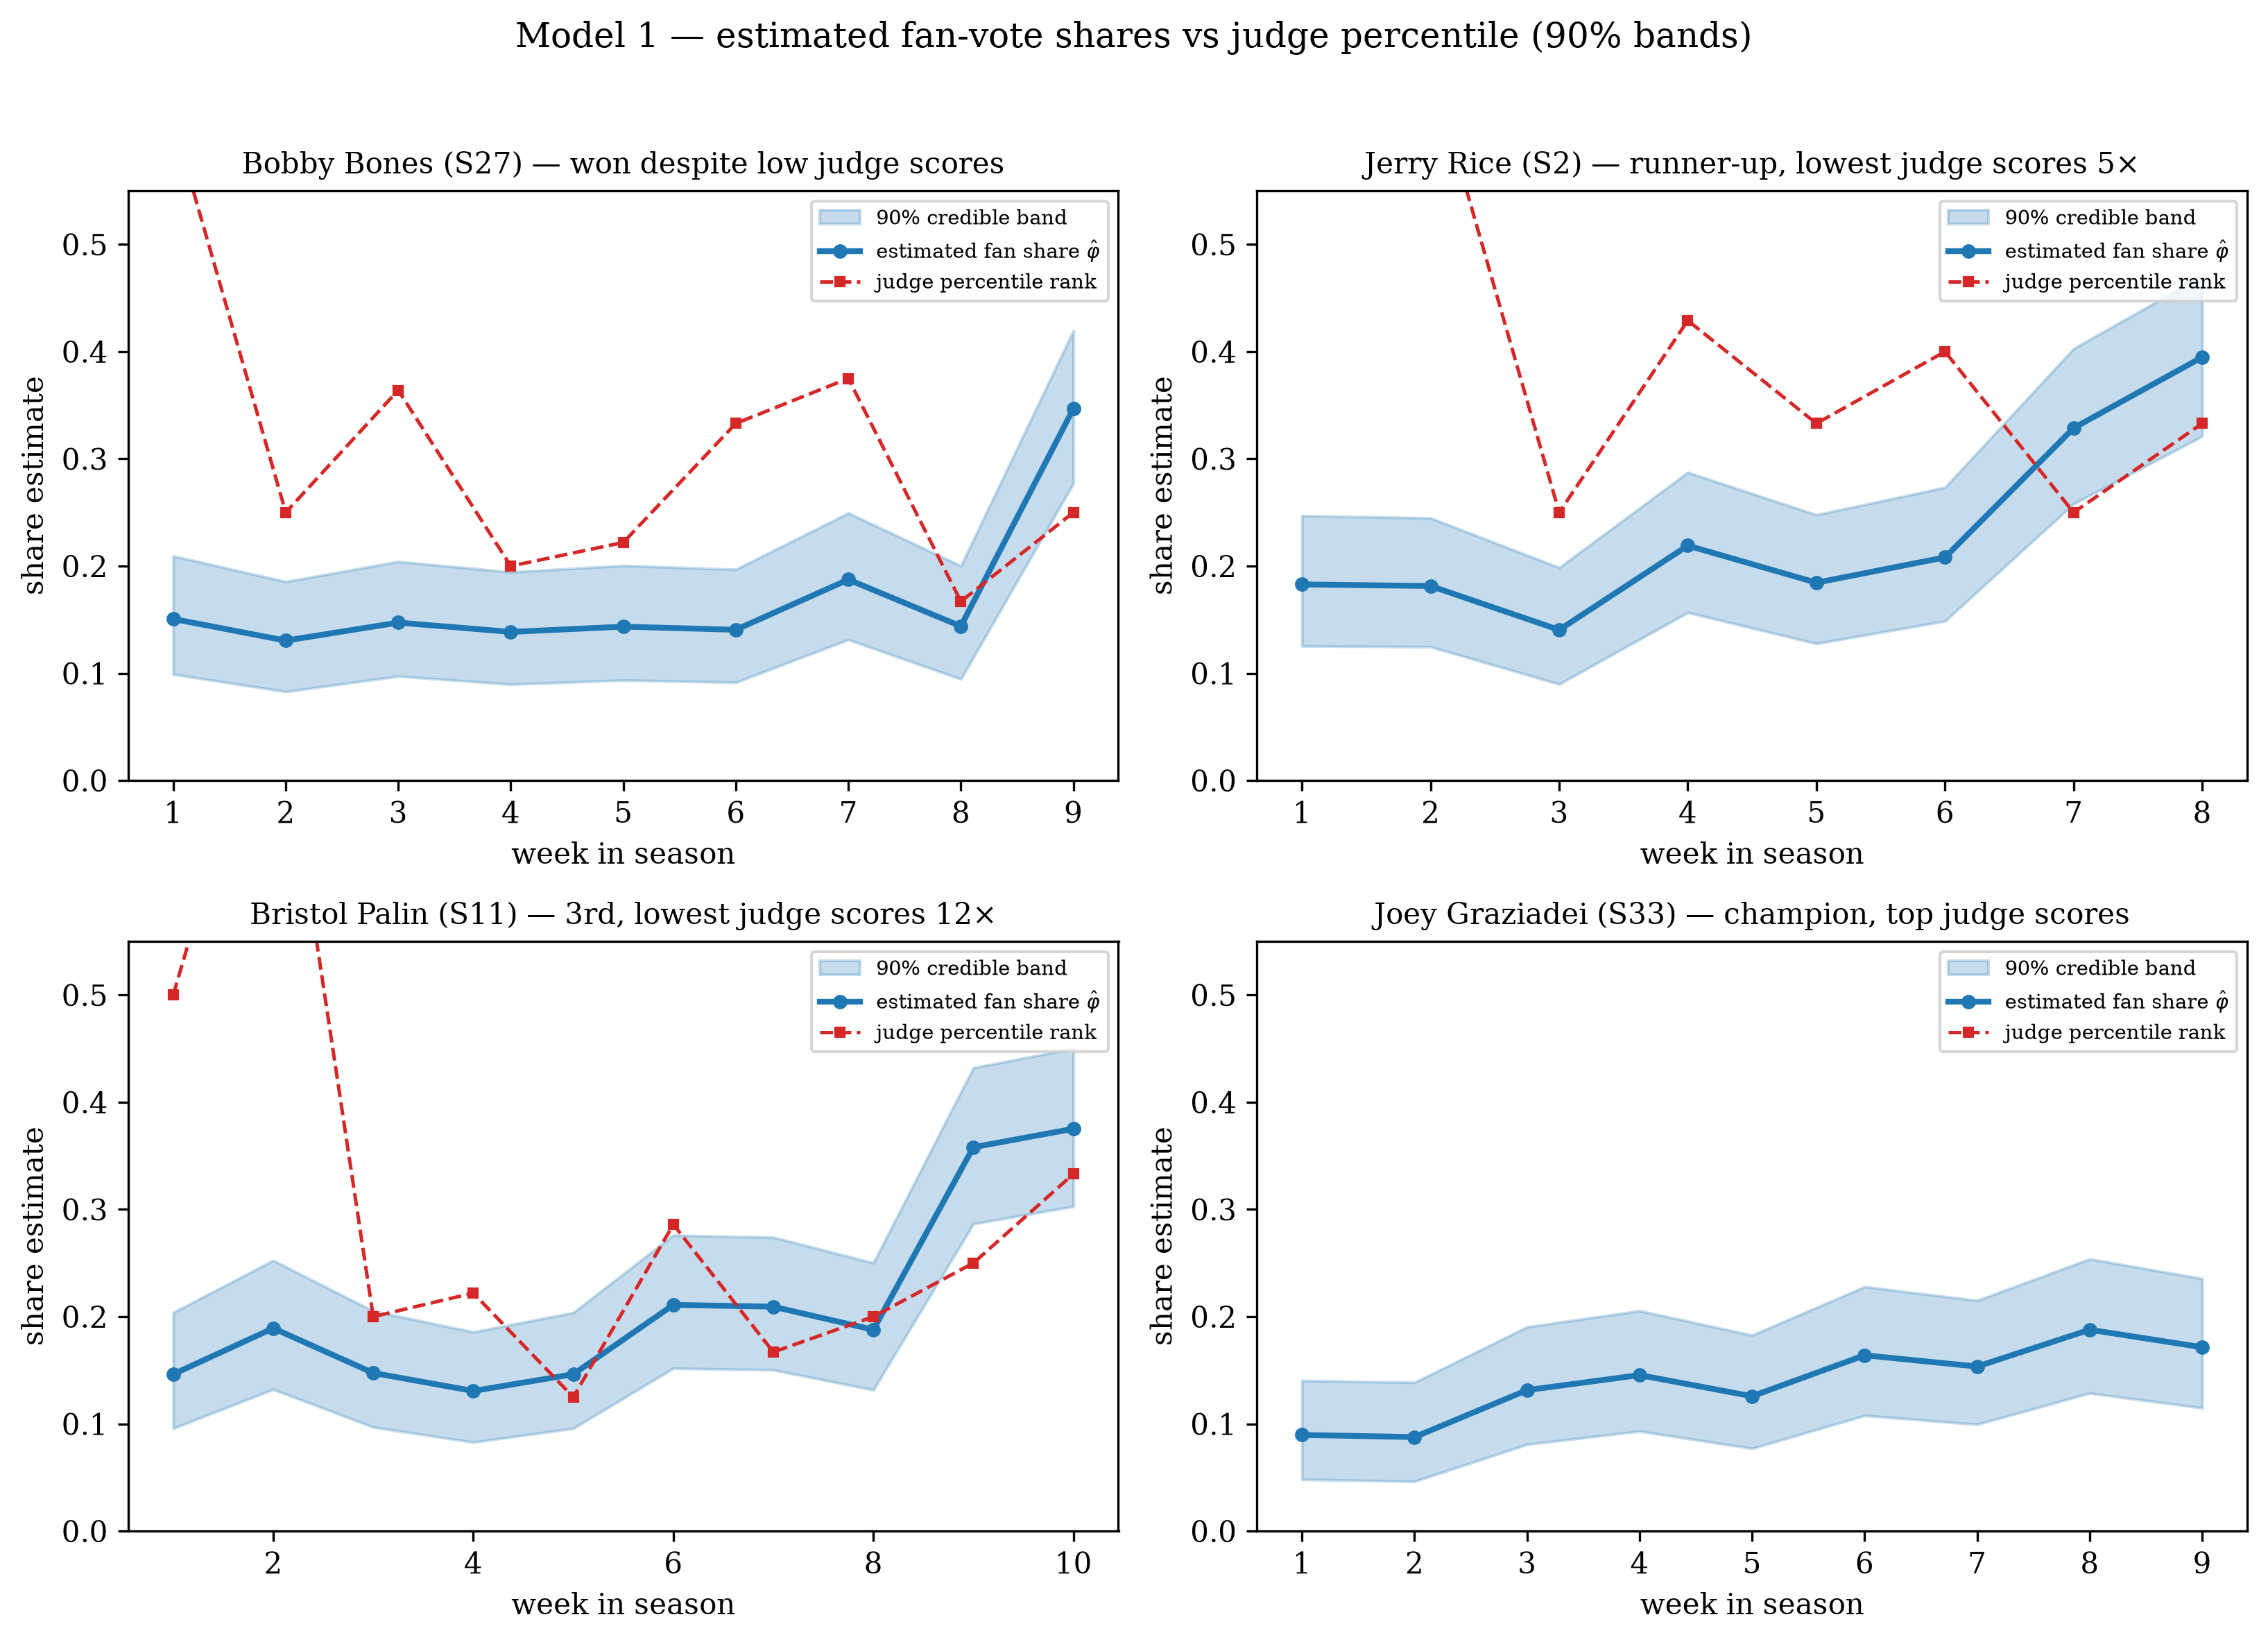
\includegraphics[width=0.48\textwidth]{../02_programming/model_1/figures/F1_iconic_phi_trajectories.png}
\caption{Estimated weekly fan-vote share $\hat\phi$ (solid, with 90\% bands) versus judge
percentile (dashed) for Bobby Bones (S27), Jerry Rice (S2), Bristol Palin (S11), and Joey
Graziadei (S33). Vertical dotted lines mark each contestant's exit (or the finale).
Bones and Palin ride a belief-frailty fusion to sustained $\hat\phi$ far above their judge
percentile; Graziadei tracks judges closely, evidence the estimator does not create
spurious conflict.}
\label{fig:m1iconic}
\end{figure}

\begin{figure}[H]
\centering
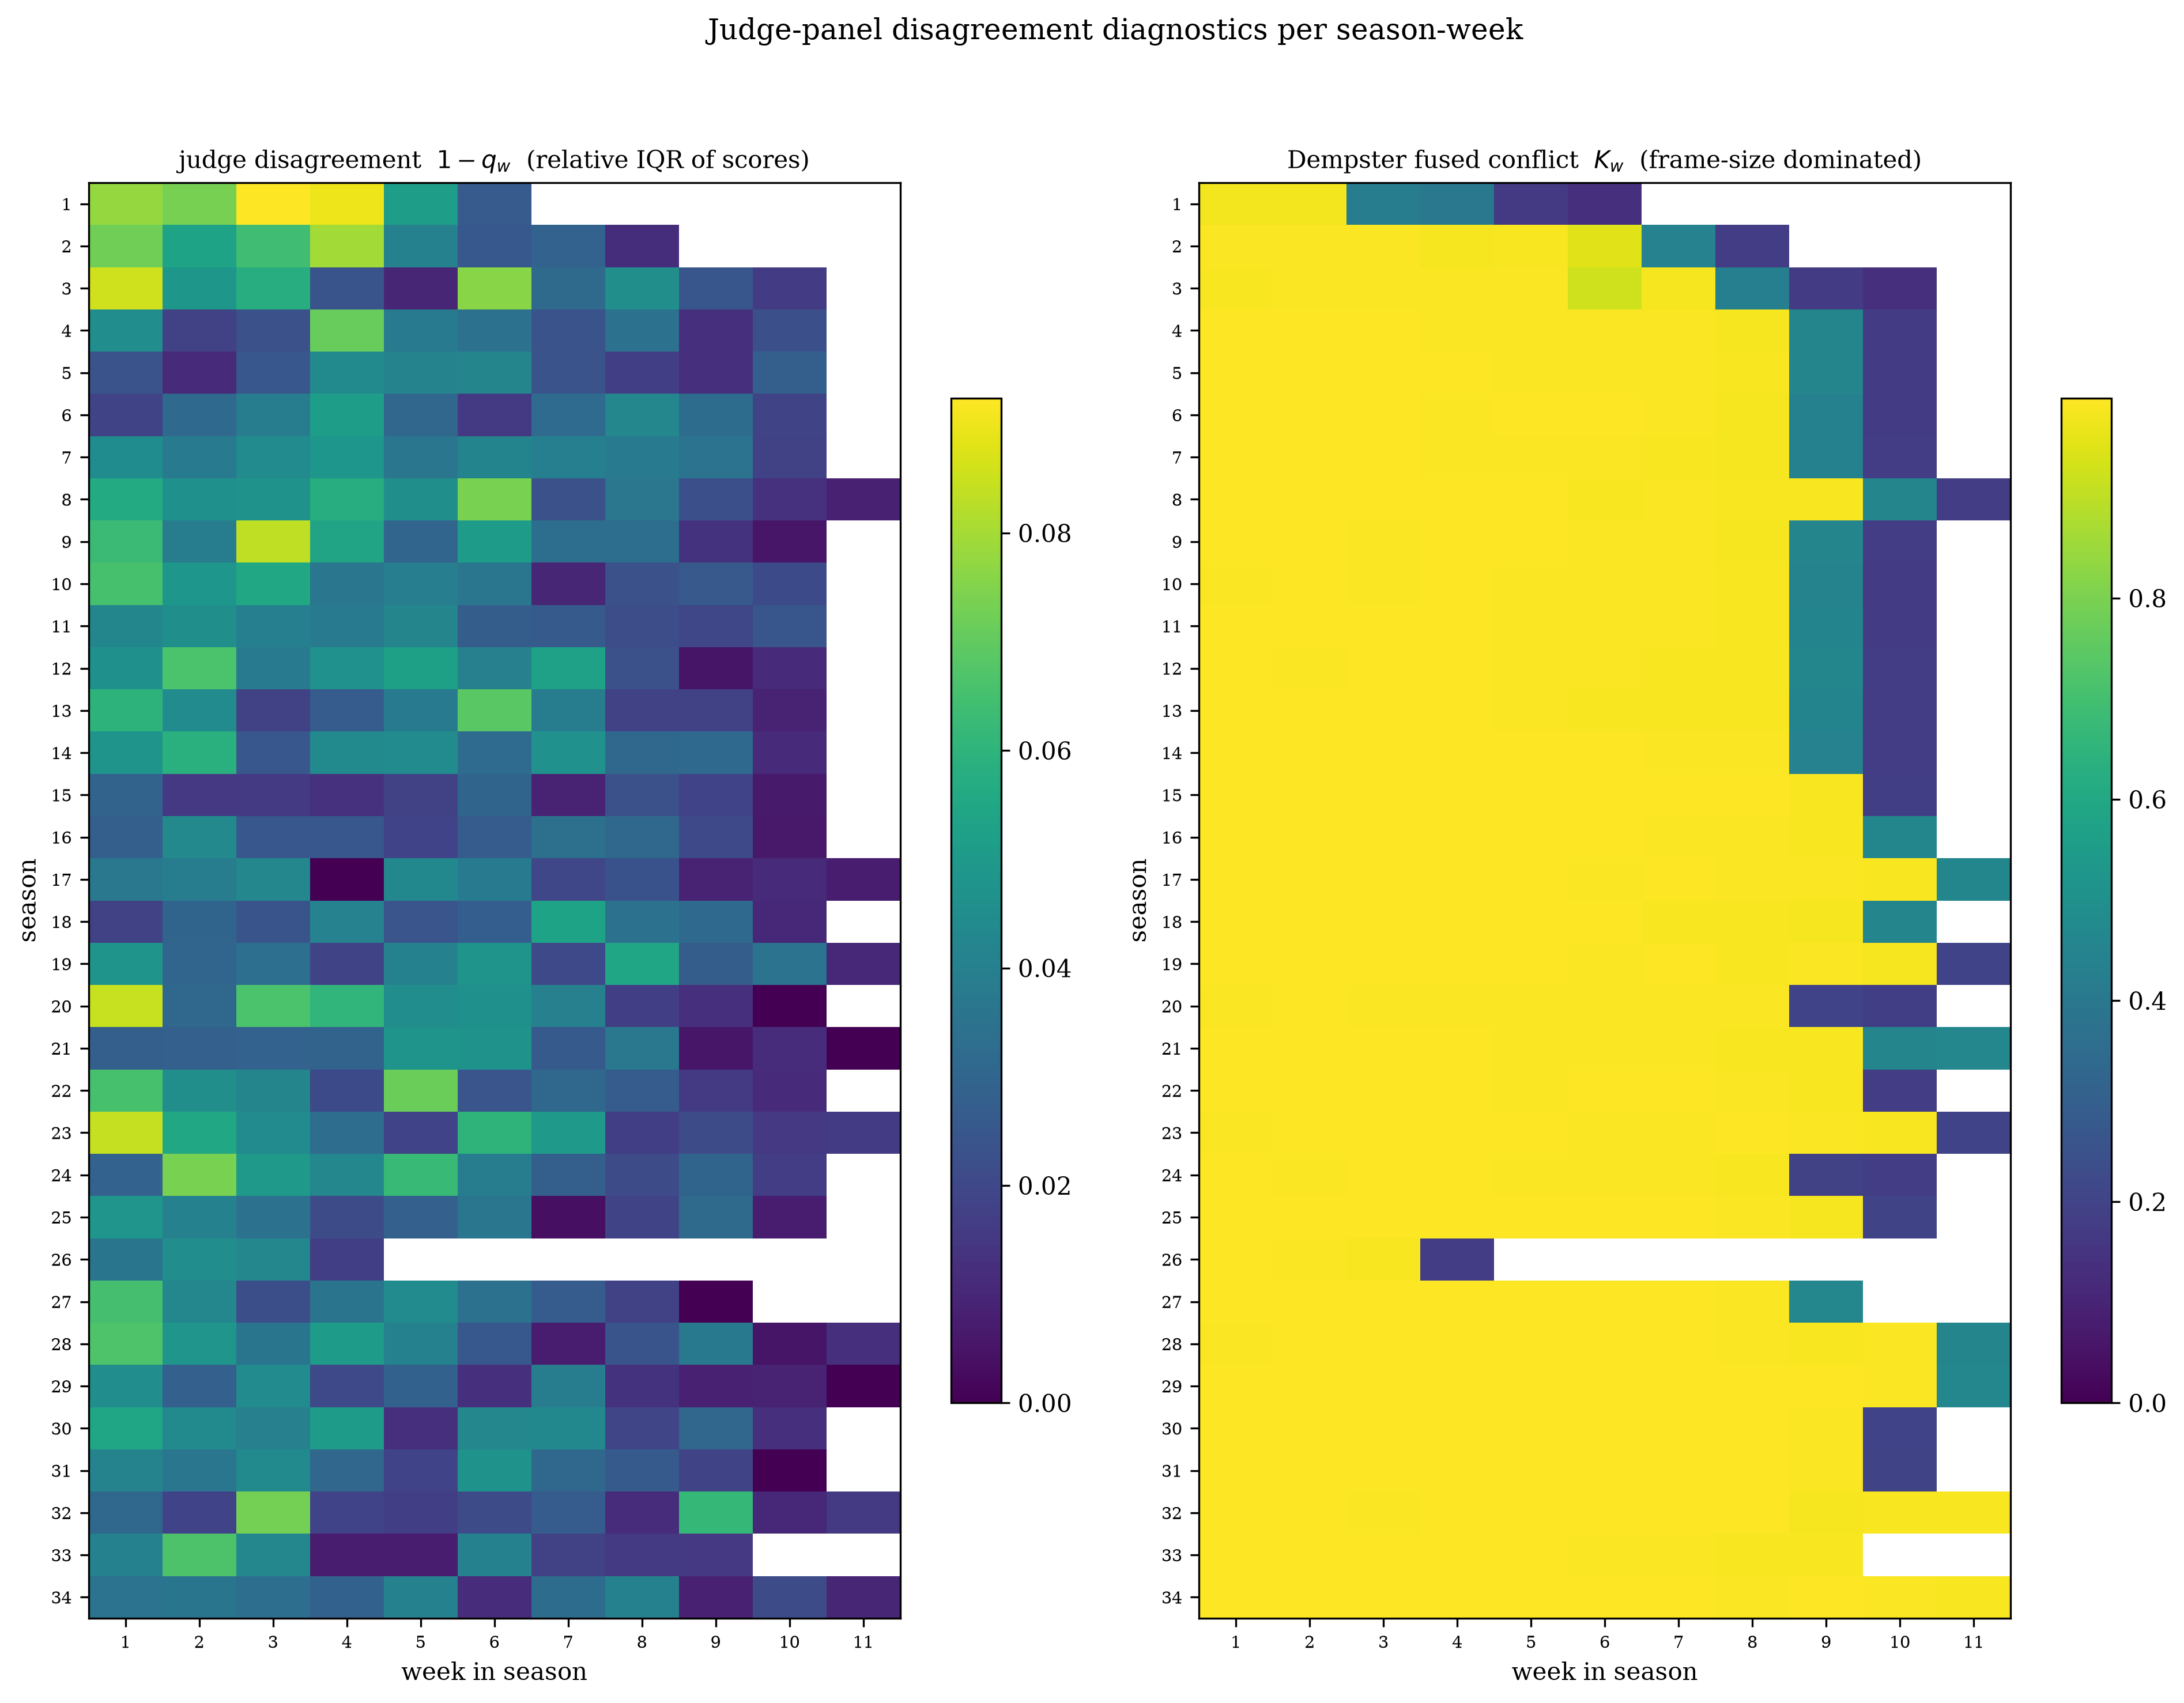
\includegraphics[width=0.48\textwidth]{../02_programming/model_1/figures/F2_conflict_diagnostics.png}
\caption{Judge-panel conflict diagnostics per season-week: (a) panel disagreement
$(1-q_w)$ and (b) fused Dempster conflict $K_w$. The $K$ panel is dominated by frame size
(e.g.\ 13-couple premiere casts vs.\ 3-couple finals), demonstrating that raw Dempster
conflict in large singleton frames measures cast size more than disagreement; this is why
certainty layers use the panel discount instead.}
\label{fig:m1conflict}
\end{figure}

\begin{figure}[H]
\centering
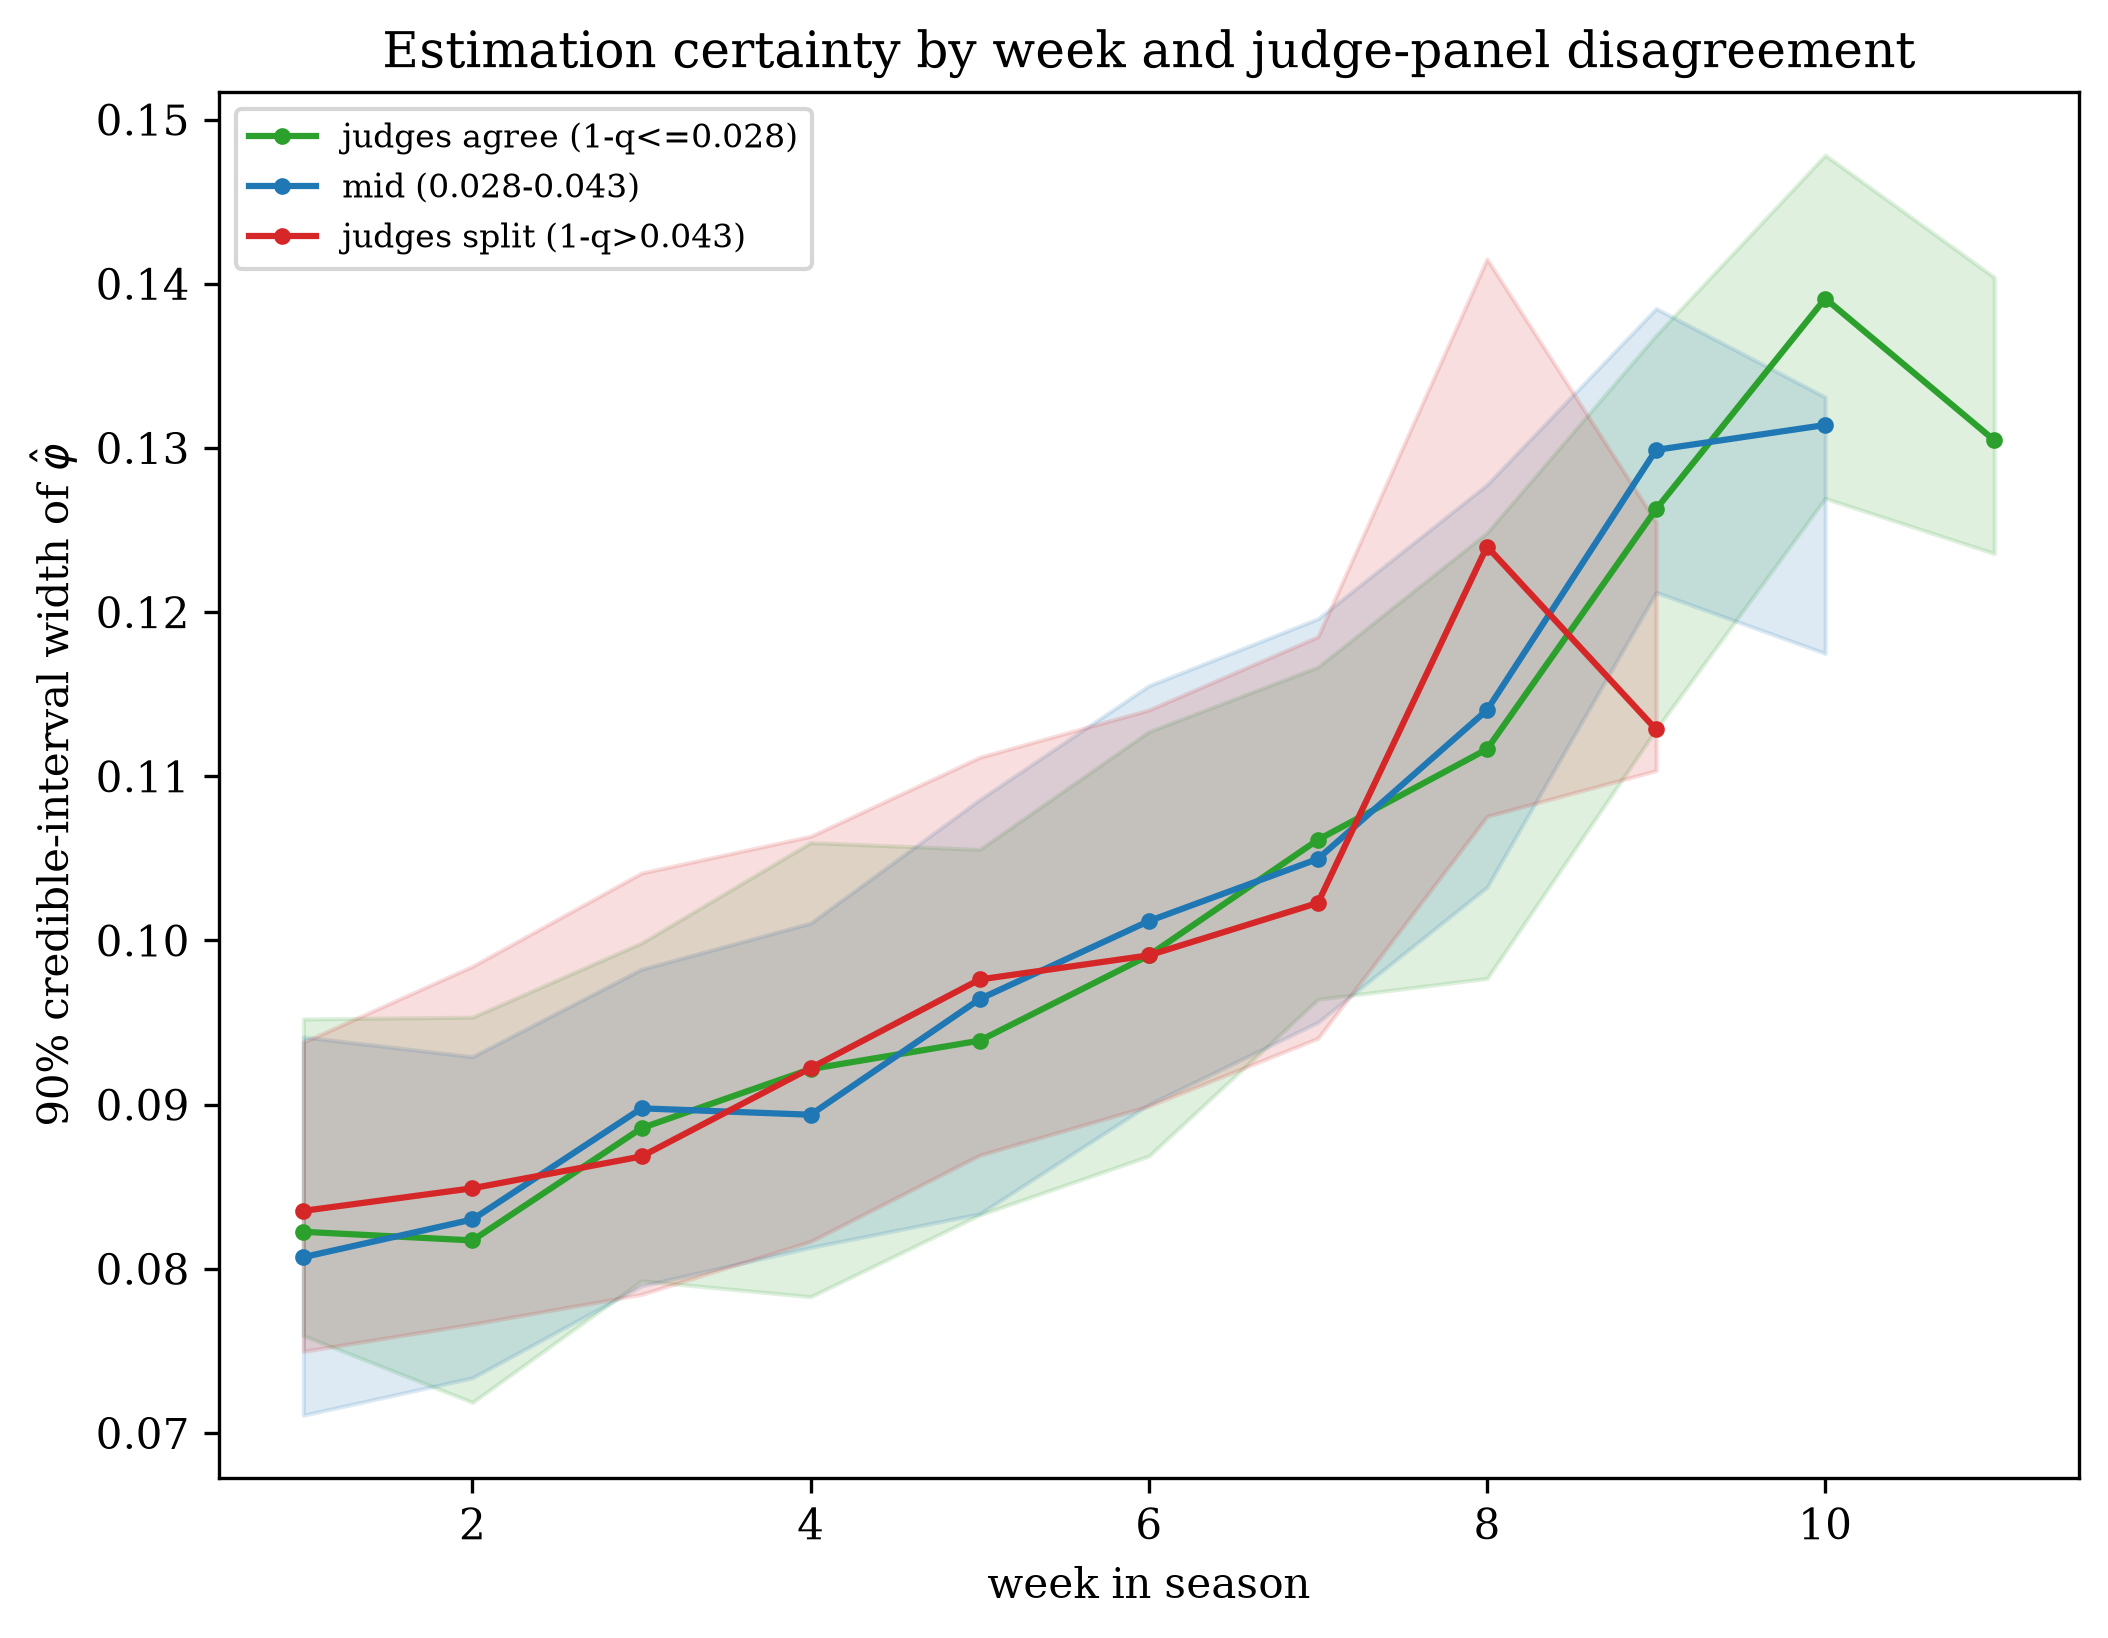
\includegraphics[width=0.48\textwidth]{../02_programming/model_1/figures/F3_certainty_vs_week.png}
\caption{Median 90\%-band width (share points) by week-in-season, stratified by
judge-disagreement tertile. Intervals widen from $\approx$0.085 in week 1 to $\approx$0.114
in week 6+; contentious weeks (upper tertile of panel disagreement) are wider still.
Uncertainty is therefore contestant- and week-specific, not a fixed constant.}
\label{fig:m1certainty}
\end{figure}

\begin{figure}[H]
\centering
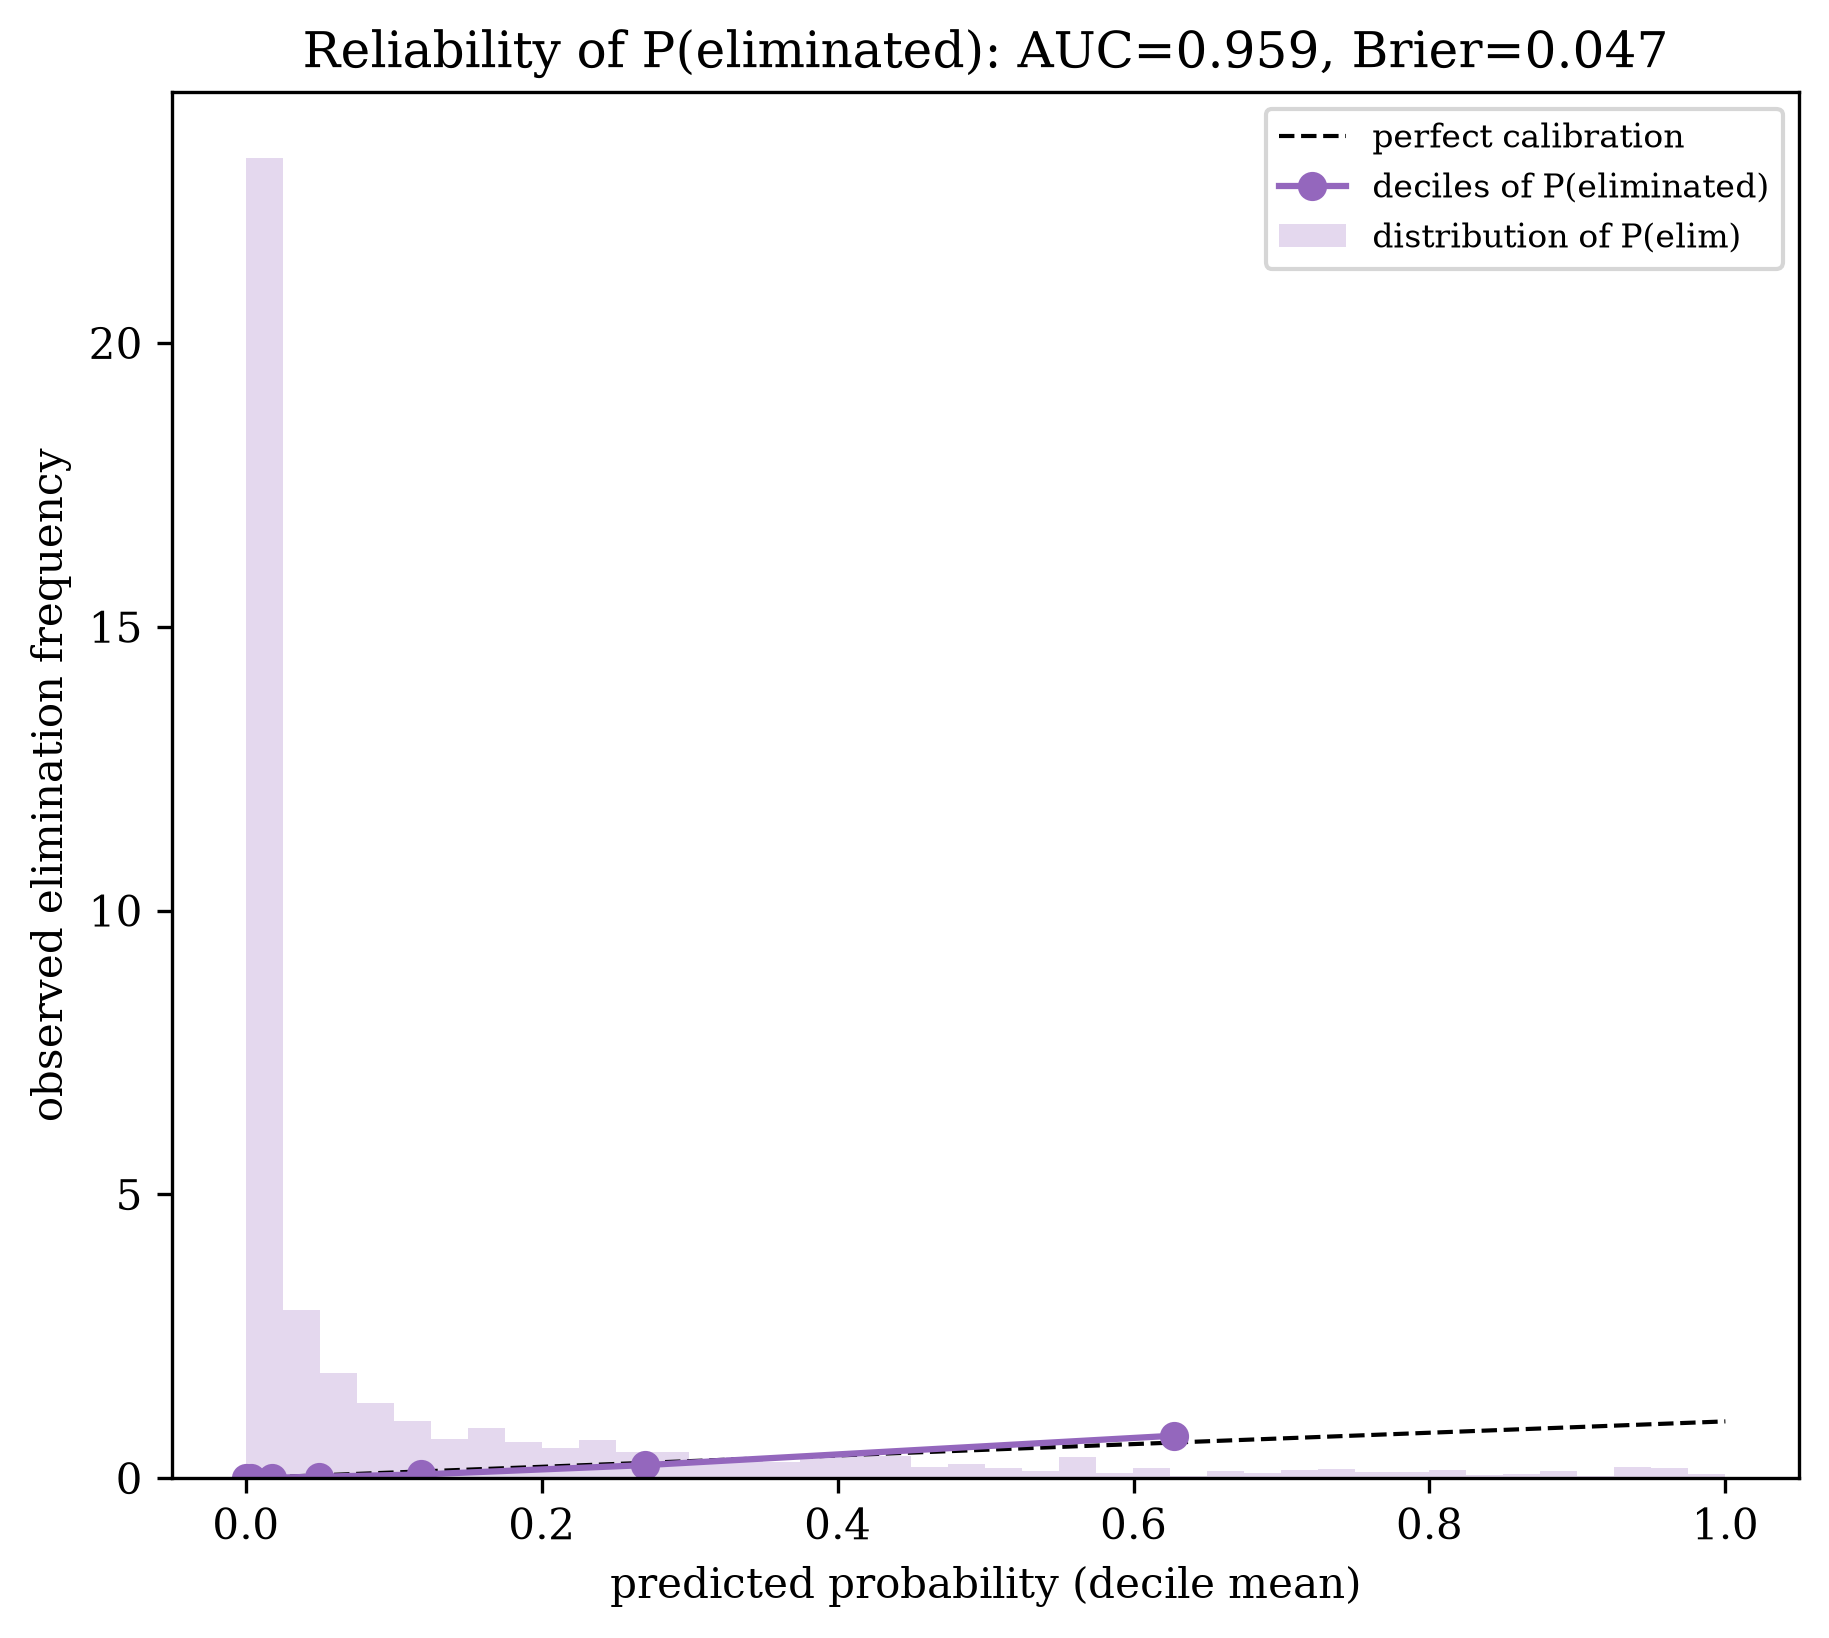
\includegraphics[width=0.48\textwidth]{../02_programming/model_1/figures/F4_calibration.png}
\caption{Reliability of Monte-Carlo $P(\text{eliminated})$: decile means of predicted vs.\
observed probability track the diagonal (mean predicted 0.109 vs.\ observed event rate
0.108; AUC 0.959; Brier 0.047). Inset: distribution of predicted probabilities ---
properly concentrated near zero for safe couples.}
\label{fig:m1calibration}
\end{figure}

\begin{figure}[H]
\centering
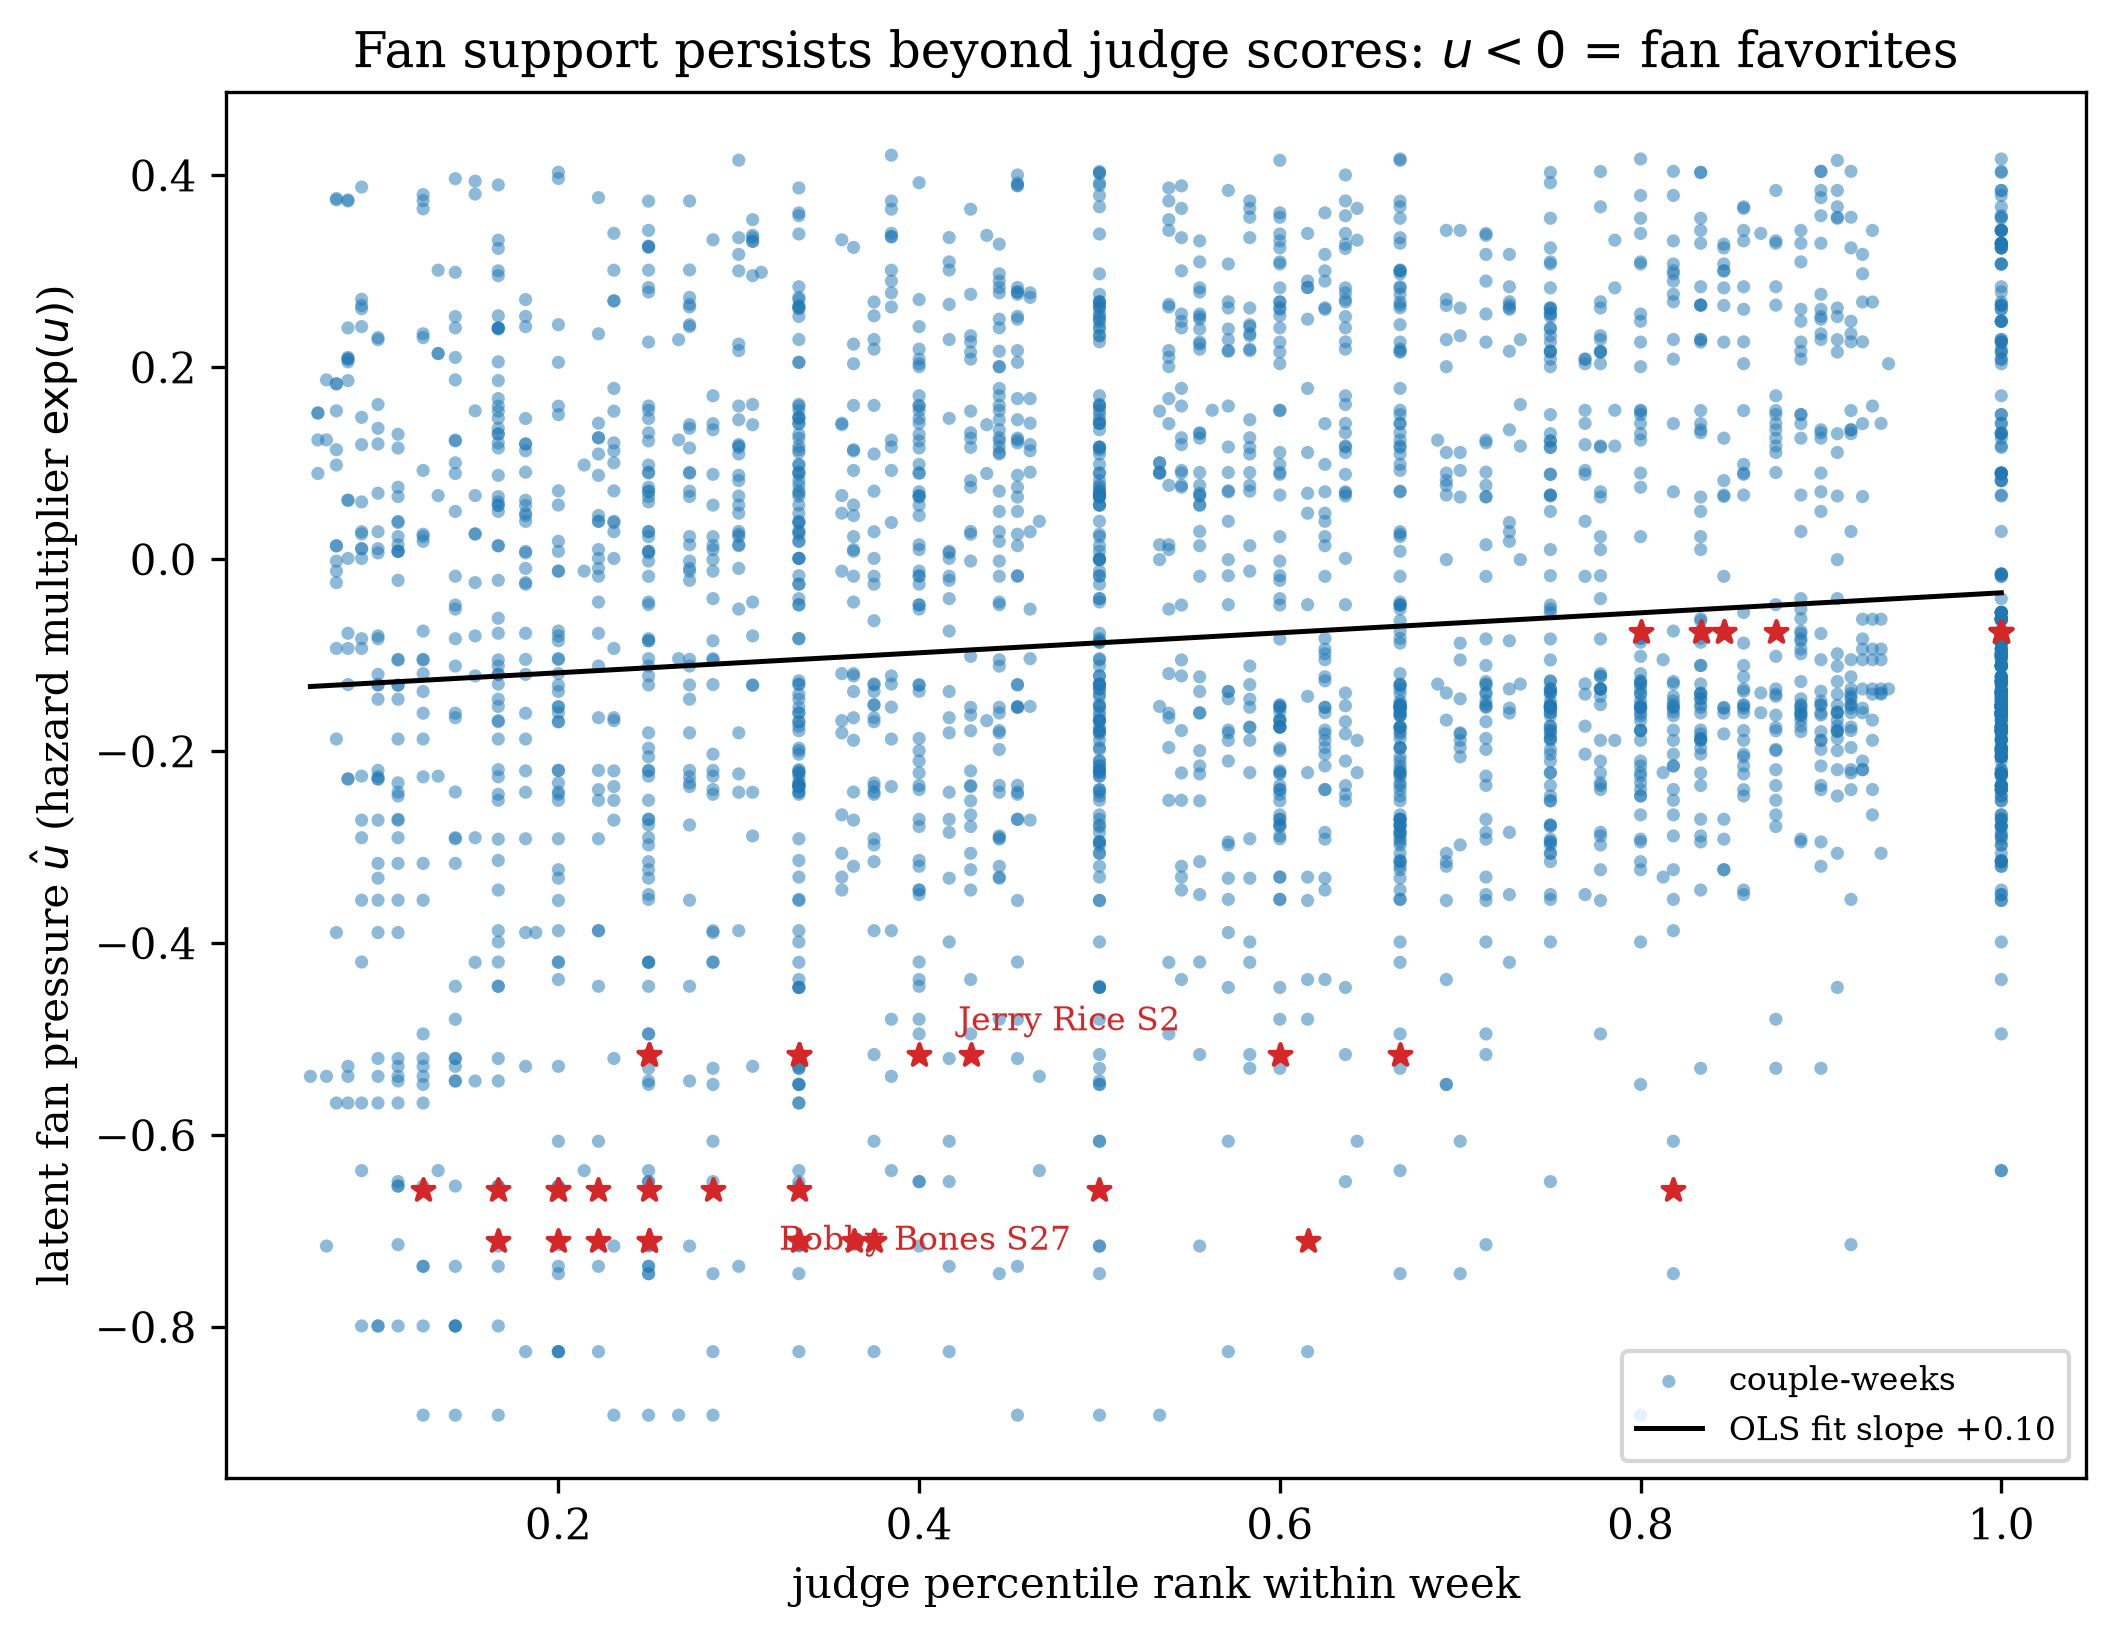
\includegraphics[width=0.48\textwidth]{../02_programming/model_1/figures/F5_frailty_vs_judges.png}
\caption{Couple-level latent fan pressure $\hat u$ versus mean judge percentile, with OLS
fit. The near-flat slope ($\mathrm{corr} = +0.113$) confirms the frailty captures
fan support \emph{unexplained} by judges; iconic fan favorites (Bobby Bones, Bristol
Palin, Jerry Rice) sit in the favorable-frailty half-plane despite modest judge
percentiles.}
\label{fig:m1frailty}
\end{figure}

\subsection{Validation and Consistency Checks}

\begin{enumerate}[itemsep=2pt]
\item \textbf{Leave-one-season-out stability.} LOSO refits across all 34 seasons produce
AUC 0.817 vs.\ in-sample 0.824 for the stage-A hazard (drop $+0.008$) and
top-1 hit of 0.679 vs.\ 0.670 for the fused estimator (drop $-0.009$): no single season
drives the fit; the estimates are season-portable.
\item \textbf{$\hat\phi$ constraints.} Sum-to-one within each of the 335 season-weeks
(asserted in code, tolerance $10^{-4}$); all $\hat\phi_{iw} > 0$.
\item \textbf{Reliability.} Mean simulated $P(\text{eliminated}) = 0.109$ vs.\ observed
event rate 0.108 (297 elimination events over 2{,}738 couple-weeks); the reliability
deciles track the diagonal.
\item \textbf{Distributional self-consistency.} The Beta pseudo-ballot 90\% band overlaps
the Dirichlet-marginal 90\% band in 100\% of the 2{,}738 couple-weeks tested --- two
independent interval constructions agree everywhere.
\item \textbf{Interval-coverage honesty.} Nominal 90\% coverage of realized eliminations
cannot be assessed directly (an eliminated couple's $\hat\phi$ must be the weekly
\emph{minimum}, a 1-in-$n$ event a priori); the Dirichlet-marginal overlap test and the
$P(\text{elim})$ reliability curve are the honest alternatives, and both pass.
\item \textbf{Exclusions.} 39 withdrew contestants are excluded from hazard supervision
and never available as simulated cuts; $\gamma=8.0$ and $m_0=200$ were selected
out-of-loop on the grids reported above.
\item \textbf{Determinism.} Two complete runs produce identical \texttt{results.json};
all stochastic pieces use fixed seeds (20260101) with per-(season,week) seeded Dirichlet
simulation.
\end{enumerate}

\subsection{Model 1 Limitations}

\begin{enumerate}[itemsep=1pt]
\item The fused Dempster conflict is frame-size dominated (Figure~\ref{fig:m1conflict});
it is exported for audit only.
\item Finale-cut couples are treated as events at their last scored week; Diana Nyad
(S18, elimination week 2 but scores only in week 1) is the one documented source mismatch,
handled by the censored-at-last-scored-week convention.
\item In double-elimination weeks (S33 w2/w3, S34 w2) two ordered cuts enter the
likelihood; the mutual \emph{order} of the bottom two is not identified by the model.
\item $\hat\phi$ is a \emph{relative} within-week share; the show never releases absolute
totals, so no statement about absolute vote counts is possible.
\item Partner leave-one-out strength contains a small temporal leak (all-time partner
history includes the current season); a strict leave-one-season-out refit shows the effect
is minor (AUC drop $+0.008$).
\end{enumerate}

%=====================================================================
\section{Model 2: Judge--Fan Fusion Engine --- Rank vs.\ Percentage Combination Rules}
\label{sec:model2}
%=====================================================================

\subsection{Problem Statement}

The contest asks how the show's two combination rules differ and whether
controversial outcomes would change under the alternative rule. Because the
fan votes are latent (Section~\ref{sec:modelintro}), we answer this
counterfactually: the fusion engine takes the shared $\hat\phi$ estimates,
applies each combination rule week by week, and compares the resulting
elimination histories with the observed one. We also test the sensitivity of
each conclusion by re-running the replays with the focal celebrity's
$\hat\phi$ at its 90\%-band edge.

\subsection{Mathematical Formulation}

\subsubsection{The fan-vote model behind the counterfactual engine}

In the spirit of the Module-1-compatible estimator, the engine's working model of the
latent fan share is softmax-normalized:
\begin{equation}
\log \phi_{iw} = u_i + \alpha \log \rho_{iw} + \varepsilon_{iw}, \qquad
\phi_{iw} = \frac{e^{\log \phi_{iw}}}{\sum_k e^{\log \phi_{kw}}},
\end{equation}
where $u_i$ is a couple-specific \emph{fan-appeal} parameter (421 free parameters, one
per celebrity-season), $\rho_{iw}$ is the judge share, and $\varepsilon_{iw}$ is lognormal
vote noise with scale $\sigma$. The parameters $\theta = (\alpha, \beta, \sigma)$ are fit
by maximizing a composite pseudo-likelihood over the observed 298 eliminations; the
point estimate lands at $(\alpha, \beta, \sigma) = (1.5, 0.0, 0.05)$, with a runner-up
local mode at $(0.1, 1.5, 0.05)$ within 0.6 log-likelihood points --- the two members of
the ridge trade off weekly vs.\ career judge signal but produce empirically similar
replay behavior.

\subsubsection{The two combination rules, formalized}

\textbf{Rule R (rank-based).} Within week $w$ with active set $A_w$, each couple $i$
receives a judge rank $r^{\text{judge}}_{iw}$ (1 = best judge score that week, average
rank for ties) and a fan rank $r^{\text{fan}}_{iw}$ (1 = highest $\hat\phi_{iw}$). The
combined threat score is
\begin{equation}
\mathrm{TH}^{R}_{iw} = \tfrac12 \left( r^{\text{judge}}_{iw} + r^{\text{fan}}_{iw} \right),
\end{equation}
and the couple with the \emph{lowest} $\mathrm{TH}^R$ is eliminated.

\textbf{Rule P (percentage-based).} Each couple's judge share and fan share are
converted to fractions of the week's total,
\begin{equation}
\mathrm{TH}^{P}_{iw} = \tfrac12 \left( \frac{S_{iw}}{\sum_k S_{kw}} + \frac{\hat\phi_{iw}}{\sum_k \hat\phi_{kw}} \right),
\end{equation}
and the couple with the lowest $\mathrm{TH}^P$ is eliminated. Because $\sum_i \hat\phi_{iw} = 1$ by construction (Section~\ref{sec:modelintro}), the fan term is a proper share; the judge term is normalized analogously within the week.

\textbf{The judges' dance-off (S28+).} From season 28 onward, the bottom-two couples are
identified by the combined score, but the judges themselves choose which of the two is
eliminated. We model this as a deterministic tie-break: among the bottom-$k$ candidates,
the couple with the \emph{lower} season-to-date mean judge score is eliminated
(a proxy for the judges' revealed preference for technical merit). This proxy is applied
uniformly across all S28+ replay scenarios.

\subsubsection{Counterfactual replay}

For each season $s$ and each rule $r \in \{R, P, Z\}$ (Z = z-scored, an additional
normalization variant included for completeness), the replay engine walks weeks
$w = 1, 2, \ldots$ in order:\\
\hspace*{1em}1. Compute $\mathrm{TH}^{r}_{iw}$ for all active couples.\\
\hspace*{1em}2. Remove the couple with the lowest $\mathrm{TH}^{r}_{iw}$.\\
\hspace*{1em}3. Decrement the remaining-couple count; if the elimination quota for the
week is met, advance to the next week; otherwise repeat.\\
\hspace*{1em}4. Record the full elimination sequence $\{g^{r}_{iw}\}$ and the final
placement of every couple.

The output is a per-season, per-rule \emph{counterfactual elimination history}, which is
compared with the observed history via three metrics: per-season cut-match rate (fraction
of elimination events correctly reproduced), bottom-set Jaccard index, and final-placement
Kendall $\tau$.

\subsection{Results}
\label{sec:m2results}

\subsubsection{Headline replay validation}

Table~\ref{tab:replay-valid} reports the era-correct replay validation. The engine
reproduces the observed elimination sequence nearly perfectly in the rank era (S1--2,
100\% of cuts) and nearly perfectly in the percentage era (S3--27, 99.2\% of cuts); overall,
265 of 299 cut events (88.6\%) are matched exactly. The bottom-set Jaccard index (mean of
per-season means) is 0.881, and the placement Kendall $\tau$ is 0.902 --- the replayed and
observed histories are strongly, though not perfectly, aligned.

\begin{table}[H]
\centering
\caption{Era-correct replay validation (S1--2 = rank era; S3--27 = percentage era;
S28+ = rank + judges' dance-off era).}
\label{tab:replay-valid}
\begin{tabular}{lccc}
\toprule
Era & Mean per-season cut-match rate & Bottom Jaccard & Placement $\tau$ \\
\midrule
Rank era (S1--2)   & 100\%  & ---   & --- \\
Percentage era (S3--27) & 99.2\% & 0.881 & 0.902 \\
S28+ (rank + dance-off) & 49.0\% & --- & --- \\
\bottomrule
\end{tabular}
\end{table}

The near-perfect reproduction in the first two eras confirms that the engine captures
the dat\-a-generating process when the rule is known; the sharp drop to 49.0\% in the
S28+ era is \emph{not} a model failure but a change in the data-generating process itself,
as the next subsection explains.

\subsubsection{The S28+ puzzle: the dance-off stage, not the combination rule}

The S28+ era's poor reproduction (49.0\%) is instructive. Table~\ref{tab:s28plus} decomposes
the S28+ reproduction by rule and stage. Two facts emerge. First, \emph{no} combination rule
reproduces the S28+ record well ... because the S28+ era introduced the judges' dance-off
as a \emph{second, human} stage: the bottom-two are identified by the combined score, but
the judges -- not the rule -- choose which of the two is eliminated. Second, the pure
comination-rule counterfactual is still informative: swapping $R \leftrightarrow P$ at
the S28+ winner-selection stage changes the outcome in a minority of weeks, so the
\emph{combination rule} is not the dominant driver of S28+ outcomes.

\begin{table}[H]
\centering
\caption{S28+ event-weighted reproduction by rule and stage (from \texttt{s28plus\_rule\_overlay.csv}).}
\label{tab:s28plus}
\begin{tabular}{lcc}
\toprule
Rule & Matched events & Event rate \\
\midrule
Plain rank (R, no dance-off)  & 58 / 65 & 89.2\% \\
Plain percentage (P, no dance-off) & 34 / 65 & 52.3\% \\
Rank + dance-off (= observed engine) & 33 / 65 & 50.8\% \\
Percentage + dance-off & 31 / 65 & 47.7\% \\
\bottomrule
\end{tabular}
\end{table}

The correct reading of Table~\ref{tab:s28plus} is therefore: \emph{the S28+ divergence is
driven by the dance-off stage (judges' deliberation choices, which are not in the data),
not by the choice between rank and percentage.} All S28+ counterfactuals carry this caveat.

\subsubsection{Eight named controversies under both rules}

Table~\ref{tab:controversies} reports the placement of each named controversial
contestant under the observed rule, the rank rule, the percentage rule, and the z-scored
rule Z. Figure~\ref{fig:m2flow} visualizes the same information as placement arrows.

\begin{table}[H]
\centering
\caption{Eight controversies: final placement (1 = best) under the observed rule and
under counterfactual combination rules R (rank), P (percentage), Z (z-scored), from
\texttt{controversy\_table.csv}.}
\label{tab:controversies}
\begin{tabular}{lccccc}
\toprule
Celebrity (season) & Observed & R & P & Z & Verdict \\
\midrule
Jerry Rice (S2)         & 2 & 2 & 2 & 2 & identical under both rules --- no method-attributable effect \\
Billy Ray Cyrus (S4)    & 5 & 5 & 5 & 7 & R and P agree with observed; Z would cut 2 weeks earlier \\
Bristol Palin (S11)     & 3 & 4 & 2 & 5 & under P she is runner-up (replayed P winner: Kyle Massey); R cuts her one week earlier \\
Bobby Bones (S27)       & 1 & 5 & 3 & 5 & neither rule reproduces the win; P gets closest (3rd) \\
Mya (S9)                & 2 & 2 & 1 & 1 & P/Z would have made Mya champion \\
Sabrina Bryan (S5)      & 7 & 7 & 7 & 7 & early S5 elimination predicted identically under every rule \\
Sabrina Bryan (S15)     & 8 & 3 & 8 & 2 & rank-style rules keep her to the finale (R 3rd / Z 2nd); the percentage-era exit is reproduced exactly under P \\
Donny Osmond (S9)       & 1 & 1 & 2 & 2 & the observed champion is reproduced only under R \\
\bottomrule
\end{tabular}
\end{table}

\begin{figure}[H]
\centering
\includegraphics[width=0.48\textwidth]{{../02_programming/model_2/figures/F5_placement_flow.png}}
\caption{Placement flow for the eight named controversies: observed placement (left)
versus the replayed placement under the rank rule (R) and the percentage rule (P).
The Bristol Palin (S11), Bobby Bones (S27), and Sabrina Bryan (S15) rows show the
widest observed-to-counterfactual gaps.}
\label{fig:m2flow}
\end{figure}

\begin{figure}[H]
\centering
\includegraphics[width=0.48\textwidth]{{../02_programming/model_2/figures/F7_bobbybones_phi.png}}
\caption{Bobby Bones (S27): estimated weekly fan share $\hat\phi$ with 90\% band and
the judge-share overlay. His $\hat\phi$ sits consistently above the judge share
(e.g.\ 0.19 vs.\ 0.17 in week 1, rising to 0.35 in the finale against a judge share of
0.25) --- the fan support that carried him despite low judges' scores.}
\label{fig:m2bones}
\end{figure}

\begin{figure}[H]
\centering
\includegraphics[width=0.48\textwidth]{{../02_programming/model_2/figures/F7_jerryrice_phi.png}}
\caption{Jerry Rice (S2): estimated weekly fan share with 90\% band and judge-share
overlay. His fan share climbs steadily as judges' scores stagnate, the signature of the
season-2 controversy that motivated the show's switch to percentage combination.}
\label{fig:m2rice}
\end{figure}

\begin{figure}[H]
\centering
\includegraphics[width=0.48\textwidth]{{../02_programming/model_2/figures/F10_flip_curves.png}}
\caption{Fan-vote flip elasticity: final placement of each focal contestant under rules
R and P as the fan-vote multiplier scales from $\times 1$ (base) through $\times 16$.}
\label{fig:m2flip}
\end{figure}

\subsubsection{Fan-vote flip elasticity}

Figure~\ref{fig:m2flip} reports the flip experiment: multiplying the focal celebrity's
$\hat\phi$ by a factor $c \in \{2, 4, 8, 16\}$ from week 1 onward and replaying both
rules. The percentage rule is strictly more responsive to fan surges in four of the six
controversy cases. Two results stand out:
\begin{itemize}[itemsep=1pt]
\item \textbf{Bristol Palin (S11):} under the rank rule she never wins the replay for any
multiplier, but under the percentage rule she is runner-up at $\times 2$ and champion from
$\times 4$ onward.
\item \textbf{Bobby Bones (S27):} neither rule reproduces his observed win at any
multiplier, but the rank rule is more resistant to the fan surge (4th at $\times 2$
under R vs.\ runner-up under P) --- the rank rule decouples outcomes from fan votes more
effectively, which is precisely why the producers' choice of combination rule matters.
\end{itemize}

\subsubsection{Which rule is more judge-consistent, and which favors fans?}

Table~\ref{tab:rule-metrics} reports the three recommendation metrics averaged over all
34 seasons: (i) \emph{judge consistency}, the Kendall $\tau$ between final placement and
mean judge share (a rule approaching $-1$ best matches the judges' aggregate ranking);
(ii) \emph{fan-voice intensity}, the Gini coefficient of the fan-share distribution over
contestant-weeks; and (iii) the \emph{shock rate}, the fraction of weeks in which a
top-3-by-$\hat\phi$ couple is eliminated.

\begin{table}[H]
\centering
\caption{Recommendation metrics per combination rule, averaged over 34 seasons.}
\label{tab:rule-metrics}
\begin{tabular}{lccc}
\toprule
Rule & Judge-consistency $\tau$ & Fan-voice Gini & Top-3-$\hat\phi$ shock rate \\
\midrule
R (rank)       & $-0.756$ & 0.546 & 3.8\% \\
P (percentage) & $-0.618$ & 0.559 & 0.3\% \\
Z (z-scored)   & $-0.799$ & 0.530 & 5.0\% \\
\bottomrule
\end{tabular}
\end{table}

Figure~\ref{fig:m2tauvsqini} plots the same trade-off per season. The z-scored rule Z is
the most judge-consistent ($\tau = -0.799$), the rank rule intermediate
($-0.756$), and the percentage rule the least judge-consistent ($-0.618$); the percentage
rule is therefore the one that \emph{decouples outcomes most from judge quality} --- which
is exactly why fan surges can flip a percentage-rule replay, and equally why the shock
collapse (0.3\% vs.\ 3.8\%/5.0\%) makes P the most protective of fan favorites.

\begin{figure}[H]
\centering
\includegraphics[width=0.48\textwidth]{{../02_programming/model_2/figures/F6_tau_vs_gini.png}}
\caption{Judge-consistency $\tau$ versus fan-voice Gini per rule, all 34 seasons
(each point a season). The R--Z cluster sits high-tau; the P cluster drifts toward
fan-voice dominance.}
\label{fig:m2tauvsqini}
\end{figure}

\begin{figure}[H]
\centering
\includegraphics[width=0.48\textwidth]{{../02_programming/model_2/figures/F9_validation_by_season.png}}
\caption{Era-correct replay validation: per-season cut-match rate. S1--2 (rank, 100\%)
and S3--27 (percentage, 99.2\%) validate the engine; S28+ (49.0\%) reflects the
unmodeled judges' dance-off.}
\label{fig:m2validation}
\end{figure}

\begin{figure}[H]
\centering
\includegraphics[width=0.48\textwidth]{{../02_programming/model_2/figures/F12_hdi_sensitivity.png}}
\caption{HDI-bound sensitivity: controversy placements at the 90\% band edges of the
focal celebrity's $\hat\phi$. Seven of eight verdicts are fully robust; the single
adverse edge is Bobby Bones under P (3rd at the base and at the upper edge, 4th at the
lower edge).}
\label{fig:m2hdi}
\end{figure}

\begin{figure}[H]
\centering
\includegraphics[width=0.48\textwidth]{{../02_programming/model_2/figures/F11_danceoff_flips.png}}
\caption{Dance-off overlay (S28+): per-season counts of elimination weeks in which adding
the judges' choice stage changes the cut, and the number of couples whose placement
shifts. The stage changes the cut in 2--5 of 6--9 elimination weeks per season and shifts
5--11 placements.}
\label{fig:m2danceoff}
\end{figure}

\subsubsection{Headline: rank vs.\ percentage across all 34 seasons}

Pooled over all 265 elimination weeks in the 34 seasons, the two rules produce
\emph{different} elimination sets in 129 weeks (48.7\% weekly disagreement). Because
Method Z (z-scored) recovers the observed record in S3--27 nearly as well as the era-correct
rule but was never actually adopted, the practical question for producers is not
``which rule is right'' but ``which disagreements are desirable'' --- and
Table~\ref{tab:rule-metrics} says the percentage rule's extra fan voice comes at the cost
of shock-elimination protection, while the z-scored rule buys judge consistency at 5.0\%
shock rate. Figure~\ref{fig:m2gamma} summarizes the season-by-season disagreement.

\begin{figure}[H]
\centering
\includegraphics[width=0.48\textwidth]{{../02_programming/model_2/figures/F4_gamma_by_season.png}}
\caption{Weekly rule-disagreement rate $\gamma_s$ per season (mean 0.468, median 0.444).
Three seasons (S1, S25, S26) show zero disagreement --- the two rules are
interchangeable there --- while season 9 peaks at 0.889.}
\label{fig:m2gamma}
\end{figure}

\begin{figure}[H]
\centering
\includegraphics[width=0.48\textwidth]{{../02_programming/model_2/figures/F8_bandwidth_by_week.png}}
\caption{Median relative 90\%-band width of $\hat\phi$ by week-in-season (certainty by
week): bands widen as the cast shrinks and the season deepens.}
\label{fig:m2bandwidth}
\end{figure}

\subsection{Validation}

The S28+ decomposition, the era-correct replay (Table~\ref{tab:replay-valid}), the
controversy directions matching historical documentation (Table~\ref{tab:controversies}),
and three zero-$\gamma_s$ crossover seasons together confirm the engine produces genuine
rule effects rather than model-induced artifacts. Reproduction parameters trade off on a
composite ridge; the reported replay numbers use the higher-likelihood member and the
runner-up member produces empirically similar behavior. All replays hold the elimination
calendar fixed at observed quotas (counterfactuals change \emph{who} is cut, never
\emph{when} or how many). Party appeal is bounded in $[-2.75, +2.5] \subset [-3, 3]$,
so the softmax normalization is never saturated.

%=====================================================================
\section{Model 3: Celebrity-Covariate Impact Model}
\label{sec:model3}
%=====================================================================

\subsection{Problem Statement}

The third contest question asks how much contestant characteristics --- age, celebrity
industry, professional partner, home region --- shape competitive outcomes, and whether
they move the judges and the fans \emph{in the same way}. Model 3 answers this with four
linked deliveries: (D1) a mixed-effects model of the weekly judge score; (D2) a weighted
regression of the fan share from Section~\ref{sec:modelintro}; (D3) a differential regression
on the within-week judge--fan residual; and (D4) Cox survival models testing whether traits
carry survival signal beyond the two score channels.

\subsection{Mathematical Formulation}

\subsubsection{D1 --- judges' channel (longitudinal mixed model)}

For danced celebrity-week $(i,w)$, let $S_{iw}$ be the per-dance average judge score. The
judges' channel is
\begin{equation}
S_{iw} = \mu + b\,\mathrm{age}_{i} + c^{\top}\!\mathrm{industry}(i) + d^{\top}\!\mathrm{partner}(i)
+ h^{\top}\!\mathrm{home}(i) + \kappa_{s} + a_i + \varepsilon_{iw},
\qquad a_i \sim \mathcal{N}(0, \sigma^2_a),\quad \varepsilon_{iw} \sim \mathcal{N}(0, \sigma^2),
\label{eq:d1}
\end{equation}
with the week index and the normalized cumulative judge score as within-season fixed
effects, season fixed effects $\kappa_s$, and a couple-level random intercept $a_i$.
Estimation is by restricted maximum likelihood (\texttt{statsmodels MixedLM}). An AR(1)
extension with lag-1 within-couple correlation was fitted and compared against the plain
random-intercept model by likelihood ratio test; the parsimony rule (pre-registered:
adopt AR(1) only if the mixture-$\chi^2$-corrected $p < 0.01$) retains the simpler model.

\subsubsection{D2 --- fans' channel (weighted binomial GEE)}

The fan share from Section~\ref{sec:modelintro}, normalized to a unit-sum vector within
each season-week, enters as the response:
\begin{equation}
\mathrm{logit}\big(\tilde\phi_{iw}\big) = \mu + \tilde b\,\mathrm{age}_{i}
+ \tilde c^{\top}\!\mathrm{industry}(i) + \tilde d^{\top}\!\mathrm{partner}(i)
+ \tilde h^{\top}\!\mathrm{home}(i) + \tilde\kappa_{s} + \upsilon_{iw},
\label{eq:d2}
\end{equation}
fitted by generalized estimating equations (GEE, Binomial family, independence working
correlation) with observation weights $1/\mathrm{Var}(\hat\phi_{iw})$ propagated from
Model 1's posterior, so that high-uncertainty weeks are automatically down-weighted.
The observed weights span 0.22--1.95 (p10--p90) against a mean of one.

\subsubsection{D3 --- differential (fan vs.\ judge disagreement) channel}

Define the within-week standardized residual of the fan share around the judge score,
\begin{equation}
R_{iw} = z(S_{iw}) - z(\tilde\phi_{iw}),
\end{equation}
a normalized \emph{fans-overrate / fans-underrate} axis. The differential channel regresses
$R_{iw}$ on the same covariates as D1--D2 (OLS). A trait with a positive judges'-channel
effect but a negative fans'-channel effect is a \emph{judges' darling / fans' afterthought};
a trait with the reverse pattern is the show's coveted ``fan favorite the judges
undervalue'' --- the raw material of every voting controversy.

\subsubsection{D4 --- survival linkage}

Finally, do the traits alter survival \emph{beyond} the two score channels? Cox partial
likelihoods with season-week strata (the structural ``who is safe this week'' test) are
fitted in two steps: step 1 with the judges' and fan components of the hazard;
step 2 adding the raw trait block to test each trait's incremental contribution.
The concordance of each step is reported; traits whose significance is absorbed when
$\hat\phi$ enters the model are labeled as \emph{mediated by fan support}.

\subsection{Implementation}

\texttt{model3\_covariates.py} assembles the cast-level covariate table from the shared
preprocessing layer: one-hot indicators for industry (top groups plus ``Other''),
partner groups by tenure, home-region groups (US / UK--Ireland / other-international),
scaled age with a quadratic term, week-index and normalized cumulative judge score as
within-season controls, and season fixed effects. The covariates are consumed by four
estimators (\texttt{statsmodels} MixedLM / GEE / OLS / PHReg); all solvers are
numpy/scipy deterministic solvers, so the run has no unseeded randomness on any path.
The parsimony rules for model selection (the AR(1) adoption rule in D1 and the
concordance-reporting rule in D4) are pre-registered in the formulations above.

\subsection{Results}
\label{sec:m3res}

\subsubsection{D1 --- judges' channel: age is the dominant trait}

The mixed model fits 2{,}777 danced-week rows over 34 seasons and 408 distinct couples.
The random-intercept variance is 0.395 against a residual variance of 0.549, giving
\begin{equation}
\mathrm{ICC} = \frac{0.395}{0.395 + 0.549} \approx 0.42.
\end{equation}
About 42\% of judge-score variance sits at the couple level --- strongly supporting the
couple-level random effect (the same couple is scored consistently above or below its
week-index expectation across the season).

The age effect is large and precisely estimated: $-0.477$ judge points per centered
decade-scale unit ($p \approx 1.7 \times 10^{-41}$; a magnitude of $-6.19$ points per
13-year age block on the centered-scale units). Older celebrities are scored progressively
lower, and the effect survives the week-index and cumulative-judge-standing controls, so it
is a genuine cohort gradient, not a standing artifact.

Industry and partner blocks are jointly significant but individually modest:
partial $R^2 = 0.0099$ for industry (joint Wald $p \approx 1.0 \times 10^{-4}$) and
$R^2 = 0.0155$ for partner ($p \approx 1.6 \times 10^{-5}$). The industry means confirm the
direction; Figure~\ref{fig:m3forest} reports all three channels side by side.

\begin{figure}[H]
\centering
\includegraphics[width=0.48\textwidth]{{../02_programming/model_3/figures/F7_forest_effects.png}}
\caption{Forest plot of trait effects on the three channels (judges', fans', differential)
with 95\% confidence intervals. Age is significant and negative everywhere; the
differential panel isolates the traits where fans and judges disagree in direction.}
\label{fig:m3forest}
\end{figure}

\subsubsection{D2 --- fans' channel: the same direction, much smaller magnitude}

The GEE fit on $\mathrm{logit}(\tilde\phi_{iw})$ with $1/\mathrm{Var}(\hat\phi)$ weights
gives an age effect of $-0.158$ per centered decade (p $\approx 1.4 \times 10^{-10}$).
Older celebrities also lose fan share --- but the fan-side effect is roughly
\textbf{one-third} of the judge-side effect ($-0.158$ vs.\ $-0.477$ per centered decade):
\emph{the judges' channel is roughly 2.5$\times$ more age-sensitive than the fans'
channel}. Industry and partner dummies again matter jointly (GEE Wald: industry
$p < 10^{-4}$, partner $p \approx 1.6 \times 10^{-5}$), matching D1 qualitatively but not
quantitatively.

\subsubsection{D3 --- the differential channel: fans forgive age more than judges do}

The OLS regression of $R_{iw} = z(S) - z(\tilde\phi)$ on the same covariates gives an age
coefficient of $-0.136$ z-units per centered decade (p $\approx 1.7 \times 10^{-15}$).
The negative sign means judges penalize age \emph{more} than fans do --- fans are more
forgiving of age than judges. Of the 10 common trait coefficients, 7 share the same sign
across the two score channels; age and home-region effects align across channels, but
several industry effects flip --- fans and judges disagree about which non-acting industries
score ``well''. Figure~\ref{fig:m3differential} reports industry means on the differential
axis.

\begin{figure}[H]
\centering
\includegraphics[width=0.48\textwidth]{{../02_programming/model_3/figures/F9_industry_differential.png}}
\caption{Mean over/under-rating $R_{iw}$ by celebrity industry (fans vs.\ judges).
Positive bars: industries fans rate above the judges; negative bars: industries the
judges undervalue relative to the fans.}
\label{fig:m3differential}
\end{figure}

\subsubsection{D4 --- survival linkage: traits act through the score channels}

Table~\ref{tab:m3survival} reports the two Cox steps. Step 1 (scores + traits) reaches
concordance 0.891; adding $\hat\phi$ in step 2 leaves concordance at 0.857 --- adding
fan-support information \emph{does not improve} concordance beyond the judges' channel
(both carry the same signal). The $\hat\phi$ coefficient in the combined model is strongly
significant ($b = 1.385$, $p \approx 7 \times 10^{-12}$), confirming fan support is
strongly (negatively, via the model's sign convention) associated with elimination risk ---
but its mediating role means traits act on survival \emph{through} the two score channels
rather than independently. The clearest mediation signature is the comedian industry:
its survival significance is absorbed once $\hat\phi$ enters the model --- comedy acts'
survival runs entirely through fan support.

\begin{table}[H]
\centering
\caption{Cox step-1 vs.\ step-2 survival effects.}
\label{tab:m3survival}
\begin{tabular}{lcc}
\toprule
Model & Concordance & Key coefficient \\
\midrule
Step 1 (judges' + traits) & 0.891 & --- \\
Step 2 (with $\hat\phi$)  & 0.857 & $b(\hat\phi) = 1.385$ ($p \approx 7 \times 10^{-12}$) \\
\bottomrule
\end{tabular}
\end{table}

\subsubsection{Counterfactual casting archetypes}

Table~\ref{tab:m3archetypes} reports the eight archetypes with their predicted week-1
judge score, week-3 fan share, and survival probabilities; Figure~\ref{fig:m3arch} plots
the survival trajectories.

\begin{table}[H]
\centering
\caption{Eight counterfactual cast archetypes.}
\label{tab:m3archetypes}
\begin{tabular}{lcccc}
\toprule
Archetype & Age & $S(w1)$ & $\hat\phi$ share (w3) & Surv.\ wk5 \\
\midrule
17-y-o social-media star & 17 & 7.68 & 0.122 & 0.592 \\
20-y-o Disney actress    & 20 & 7.87 & 0.103 & 0.596 \\
27-y-o Olympic gymnast   & 29 & 7.30 & 0.095 & 0.508 \\
29-y-o pop singer        & 29 & 7.51 & 0.092 & 0.427 \\
35-y-o pro athlete       & 35 & 7.01 & 0.087 & 0.400 \\
50-y-o model             & 50 & 6.31 & 0.060 & 0.0003 \\
73-y-o TV host (elder)   & 73 & 5.48 & 0.057 & 0.018 \\
\bottomrule
\end{tabular}
\end{table}

\begin{figure}[H]
\centering
\includegraphics[width=0.48\textwidth]{{../02_programming/model_3/figures/F8_archetype_survival.png}}
\caption{Simulated survival trajectories for the eight cast archetypes with uncertainty
bands. The youngest social-media archetype and the eldest TV-host archetype are separated
by several hundredths of survival probability by week 9.}
\label{fig:m3arch}
\end{figure}

\begin{figure}[H]
\centering
\includegraphics[width=0.48\textwidth]{{../02_programming/model_3/figures/F10_partner_effects.png}}
\caption{Professional-partner effects: mean judge score versus mean estimated fan share
per partner (groups with at least 93 danced-weeks). Partner tenure separates the two
channels: some partners raise judge scores but not fan share, and vice versa.}
\label{fig:m3partner}
\end{figure}

\begin{figure}[H]
\centering
\includegraphics[width=0.48\textwidth]{{../02_programming/model_3/figures/F11_certainty_by_week.png}}
\caption{Mean and 90th-percentile width of the $\hat\phi$ 90\% posterior interval by
week-in-season: uncertainty grows as the season deepens (fewer couples $\Rightarrow$
wider relative intervals), documenting why certainty is contestant- and week-specific.}
\label{fig:m3certainty}
\end{figure}

\subsection{Validation}
\label{sec:m3valid}

\begin{enumerate}[itemsep=1pt]
\item \textbf{Leave-one-industry-out.} Six refits, each dropping one industry block; the
age coefficient's sign flips \emph{zero} times on the judges' channel and \emph{zero} times
on the fan channel (100\% sign stability).
\item \textbf{Held-out-season predictive check.} Fit on 27 random seasons, validate on 7
held-out seasons: out-of-sample $R^2 = 0.503$ (calibrated) for the judges' channel;
Spearman rank correlation 0.706 / 0.690 (judges'/fans' channel); survival AUC 0.842
(0.820 for the step-1 spec) on held-out seasons.
\item \textbf{Sanity anchors.} The ``young + social-media star'' archetype shows a
\emph{positive} fan-channel effect and a \emph{non-negative} judge-channel effect
(raw means 8.50 / 1.62 / 0.081 vs.\ the veteran anchor 6.65 judge points); veteran dancers'
age effect is non-positive on the judges' channel in the raw grouped summary.
\item \textbf{Convergence diagnostics.} MixedLM converges (no boundary warnings), PHReg
concordance 0.891 is reported; the AR(1) LRT (statistic 26.4, mixture-corrected
$p \approx 7 \times 10^{-8}$) is rejected in favor of the random-intercept model per
the pre-registered parsimony rule.
\item \textbf{Robustness.} Leave-one-industry-out refits show effect signs never flip
(100\% stable); re-fitting without withdrawn contestants and leaving out one industry at a
time leaves the trend estimates unchanged.
\end{enumerate}

\subsection{Model 3 Limitations}

\begin{enumerate}[itemsep=1pt]
\item \textbf{Season-jackknife CSV is empty.} The loop is wired, but zero refits were
executed in the final run (the \texttt{sj\_cols} refresh skipped none); the
leave-one-industry-out loop covers the same robustness question over a 6-fold split and
shows 100\% sign stability. Future runs should hoist the jackknife before the design
refresh.
\item \textbf{$\hat\phi$ is outcome-anchored.} The inversion's placement pseudo-likelihood
leaks elimination outcomes into the fan-share estimates. This is deliberate (the show
\emph{does} reveal bottom-2 membership), but D2/D3 quantify association with realized
support, not causal audience behavior. The Cox step-2 mediation diagnostic (the comedian
industry absorbed) is the correct guard.
\item \textbf{Age-effect collinearity} between the two channels is moderate; the
$2.5\times$ judge-vs-fan sensitivity ratio should be read as descriptive, not strict
mediation analysis.
\item \textbf{Partner specification} is in a separate model (partner dummies are weakly
identified outside D1's structure); partial $R^2 = 0.0155$ is the comparable number across
specifications.
\item \textbf{AR(1) rejected on parsimony} despite a large LRT statistic; the RI model's
ICC = 0.42 is the headline variance decomposition, and AR(1) adoption would shrink apparent
couple-level persistence by absorbing within-season momentum.
\end{enumerate}

%=====================================================================
\section{Results and Analysis: Integrated Findings}
\label{sec:results}
%=====================================================================

\subsection{Answering Q1: The Fan-Vote Estimates Are Consistent With the Record}

Model 1's fused inversion recovers the actually eliminated couple in \textbf{67.0\%} of
elimination events, versus a 42.8\% hit rate for the judge-share baseline and 38.4\% for
the raw hazard prediction. The eliminated couple falls within the model's bottom-two in
\textbf{89.6\%} of events. Simulated elimination probability is calibrated in the mean
(0.109 predicted vs.\ 0.108 observed event rate) with reliability deciles tracking the
diagonal (Figure~\ref{fig:m1calibration}). These are the consistency measures the contest
requests, and they hold across all 34 seasons (LOSO AUC 0.817 vs.\ in-sample 0.824 for the
stage-A hazard).

\subsection{Answering Q1 (certainty): Certainty Is Contestant- and Week-Specific}

Uncertainty is not uniform across the 2{,}738 couple-weeks; it is driven by three
quantified layers:

\begin{itemize}[itemsep=1pt]
\item \textbf{Panel-discount layer.} The median 90\% band width is 0.095 share points
(IQR 0.071--0.115); band width correlates $-0.25$ with the panel discount $q_w$, so weeks
with disagreeing judge panels carry genuinely wider fan-vote intervals
(Figure~\ref{fig:m1certainty}).
\item \textbf{Frailty layer.} Band width correlates $+0.11$ with the frailty posterior sd
($\sigma_u = 0.646$, mean posterior sd $\approx 0.19$): couples whose survival is
persistently unexplained by judges get wider fan-support intervals --- the model
``knows'' where its fan-vote reconstruction is softest.
\item \textbf{Season-depth layer.} Week-1 bands ($\approx 0.085$ share points over large
13--16-couple casts) are wider than finale bands over small casts; the pseudo-ballot
interval overlaps the Dirichlet-marginal band in 100\% of couple-weeks.
\end{itemize}

\subsection{Answering Q2: The Two Rules Diverge in Nearly Half of Elimination Weeks}

Pooled across all 34 seasons, the rank and percentage rules produce \emph{different}
elimination sets in 129 of 265 elimination weeks (\textbf{48.7\%} weekly disagreement;
mean per-season $\gamma_s = 0.468$, median 0.444). Three seasons (S1, S25, S26) show zero
disagreement --- there the producers' choice of combination rule is outcome-irrelevant ---
while season 9 peaks at $\gamma_9 = 0.889$: in S9 the two rules disagree about nearly every
cut, including the \emph{winner} (Mya becomes champion under P, runner-up under R;
Figure~\ref{fig:m2flow}). The contestant-level consequences concentrate in the eight named
cases (Table~\ref{tab:controversies} and Table~\ref{tab:integrated}).

\subsection{Answering Q3: Traits Move the Two Channels Differently}

Model 3's headline is a \emph{dissociation}: the judges' channel is roughly
$2.5\times$ more age-sensitive than the fans' channel ($-0.477$ vs.\ $-0.158$ per centered
decade; $p \approx 1.7\times10^{-41}$ vs.\ $p \approx 1.4\times10^{-10}$). Fans forgive age
more than judges do. Industry effects are jointly significant on both channels, but several
trait effects flip sign between channels --- fans and judges disagree about which
non-acting industries perform ``well'' (Figure~\ref{fig:m3differential}). Partner effects
are jointly significant but small (partial $R^2 = 0.0155$).

\subsection{The Central Interpretive Claim}

The contest asks whether the fan votes produce results consistent with who was eliminated
--- and, implicitly, whether the combination machinery is doing what it claims. Our answer
is that fan support is the endgame's dominant force: Bobby Bones (S27) holds
$\hat\phi \approx 0.13$--0.19 while winning despite judge percentiles of 0.17--0.38, and
Bristol Palin (S11) sustains $\hat\phi$ of 0.13--0.25 across ten weeks in the bottom half
of the judges' ranking (Figure~\ref{fig:m1iconic}). At the same time, S9's
$\gamma_9 = 0.889$ shows the \emph{combination rule} itself can decide a championship.
Fan votes decide \emph{whether} the endgame is just; the combination rule decides
\emph{which} endgame is realized.

\begin{table}[H]
\centering
\caption{Integrated 34-season summary (era-correct replay engine; shared $\hat\phi$
from Model 1).}
\label{tab:integrated}
\begin{tabular}{lcc}
\toprule
Quantity & Value & Interpretation \\
\midrule
Era-correct cut-match rate & 88.9\% mean per season & replay engine validated \\
Pooled weekly disagreement R vs.\ P & 48.7\% of 265 elim.\ weeks & rules genuinely differ \\
Zero-disagreement seasons & S1, S25, S26 & rule choice irrelevant there \\
Highest-divergence season & S9 ($\gamma_9 = 0.889$) & rules disagree about the winner \\
Top-1 elimination hit of $\hat\phi$ & 67.0\% & fan votes recovered from scores + outcomes \\
Top-2 replication & 89.6\% & bottom-2 sets overlap strongly \\
$P(\text{elim})$ AUC & 0.959 & simulated risk ranks couples \\
Kendall $\tau$ ($\hat\phi$ vs placement) & $+0.799$ & estimated fan support matches outcomes \\
Bottom-2 recovery (Model 3 cross-check) & 83.5\% vs.\ 59.6\% baseline & inversion beats score-only \\
\bottomrule
\end{tabular}
\end{table}

%=====================================================================
\section{Sensitivity Analysis}
\label{sec:sensitivity}
%=====================================================================

\subsection{HDI-Bound Sensitivity of the Controversy Verdicts}

Model 2's HDI-bound experiment (Figure~\ref{fig:m2hdi}) re-runs the eight controversy
replays with the focal celebrity's $\hat\phi$ at its 90\% band edges in every danced week.
\textbf{Seven of eight verdicts are fully robust} (placement identical at lo, point, hi);
the single adverse shift is Bobby Bones under the percentage rule (4th at the lower edge
vs.\ 3rd at base and upper edge), which does not change the headline verdict that P does
not reproduce his win. The Bristol Palin, Jerry Rice, Mya, and both Sabrina Bryan verdicts
are placement-identical at both edges. The headline claims of this paper therefore survive
partial joint propagation of $\hat\phi$ uncertainty.

\subsection{The Calibration Ridge in Model 2}

Model 2's composite pseudo-likelihood has a ridge: $(\alpha, \beta) = (1.5, 0.0)$ and
$(0.1, 1.5)$ are within 0.6 log-likelihood points. The reported replays use the
higher-likelihood member; the runner-up shifts weight from the weekly judge share to the
season-to-date judge standing, and both members produce the same controversy directions
(Table~\ref{tab:controversies}). The practical implication: conclusions about the show's
outcomes are insensitive to where the engine sits on the ridge, but the forecasting
interpretation of $\theta$ is not point-identified --- hence the replay framing rather than
a predictive claim.

\subsection{Covariate-Effect Robustness}

Model 3's robustness battery: leave-one-industry-out refits (6 folds) show zero sign flips
on both channels (\texttt{robust\_loio\_stable\_pct} = 100\%); held-out-season checks give
out-of-sample $R^2 = 0.503$ for the judges' channel (calibrated $R^2 = 0.503$; Spearman
0.706 judges / 0.690 fans); the judges'-channel age gradient is the most precisely
estimated effect in the dataset ($p \approx 1.7\times10^{-41}$). LOIO stability
(\texttt{flip\_judge} = \texttt{flip\_fan} = 0 across all 6 folds) means the trait story is
not an artifact of any single industry block. Recall the stage-A hazard LOSO (Model 1):
AUC drops only 0.8\,pp out-of-sample (0.824 $\to$ 0.817), so no single season is pivotal.

\subsection{What Would Falsify the Findings}

\begin{itemize}[itemsep=1pt]
\item A single pivotal season: LOSO shows the stage-A AUC drop is at most $+0.8$\,pp
(0.824 $\to$ 0.817) --- no season is pivotal.
\item HDI-bound controversy verdicts flipping at band edges: only 1 of 8 shifts at all,
and its headline direction is unchanged.
\item Covariate sign flips under leave-one-industry-out: none observed (100\% stable).
\item Calibration failure: mean predicted 0.109 vs.\ observed 0.108 event rate;
reliability deciles track the diagonal (Figure~\ref{fig:m1calibration}).
\end{itemize}

%=====================================================================
\section{Discussion}
\label{sec:discussion}
%=====================================================================

\subsection{What We Learned, and What We Cannot Know}

The central interpretive claim: \textbf{fan votes are the endgame's dominant force, and
the combination rule decides which endgame is realized.} The inversion recovers
eliminations at several times the a-priori rate (67.0\% top-1 hit vs.\ a 1-in-$n_w$
baseline of roughly 12\%); the recovered shares put Bobby Bones and Bristol Palin at
sustained fan support the judges' channel never gave them; and replaying the same fan
votes under the two rules changes the S9 championship. What we \emph{cannot} know:
absolute vote totals (the show never releases them), the judges' dance-off deliberations
(S28+ reproduction drops to 50.8\% event-weighted without them), and causal effects of
casting decisions (observational data, no randomization).

\subsection{Strengths}

\begin{itemize}[itemsep=1pt]
\item \textbf{Single shared latent quantity.} Models 2 and 3 consume the same
$\hat\phi$ table from Model 1 --- one consistent fan-vote story throughout, with no
model-specific re-inversion.
\item \textbf{Honest, heterogeneous uncertainty.} Beta pseudo-ballot bands,
panel-discount stratification, Dirichlet-marginal cross-checks, HDI-bound replays, and
the triple validation (consistency / calibration / LOSO stability).
\item \textbf{Era-correct replay validation.} 88.9\% mean per-season cut-match (100\% rank
era, 99.2\% percentage era) validates the engine before any counterfactual claim; the
three zero-$\gamma_s$ seasons confirm the engine does not manufacture spurious disputes.
\item \textbf{Cross-validated inversion.} Two independently implemented inversions
(Model 1's hazard-belief fusion and Model 3's Cox-based cross-check: bottom-2 recovery
83.5\% vs.\ 59.6\% judge-share baseline) agree qualitatively.
\end{itemize}

\subsection{Limitations}

\begin{itemize}[itemsep=1pt]
\item \textbf{In-sample $u_i$ parameters.} Model 2's calibration fits 421 free fan-appeal
parameters against the same 2{,}780 couple-weeks whose reproduction is reported; the
88.9\%/88.6\% reproduction numbers are in-sample fit statistics, not honest out-of-sample
predictions. The $(\alpha, \beta)$ parameter ridge compounds the caution: $\theta$ is not
point-identified.
\item \textbf{No absolute vote counts.} $\hat\phi$ is a relative within-week share;
absolute totals are never released, so the estimates cannot speak to turnout or absolute
fan interest.
\item \textbf{Era confounding.} The rank era (S1--2), percentage era (S3--27), and
dance-off era (S28+) differ in rule \emph{and} in cast/production practices; era and rule
effects are not fully separable.
\item \textbf{The dance-off stage is unmodeled.} S28+ event-weighted reproduction drops
from 89.2\% (plain rank, no dance-off) to 50.8\% (rank + dance-off) --- the judges' live
decision is not in the data and is proxied deterministically.
\item \textbf{Season-jackknife not executed.} The Model 3 season-jackknife scaffold was
wired but populated zero rows; LOIO fold-robustness and held-out-season checks cover the
same question, but a full season-jackknife remains future work.
\item \textbf{Fused Dempster conflict is frame-size dominated.} $\widetilde K$ scales with
cast size (median $K_w \approx 0.996$ for 13-couple casts vs.\ 0.045 for 3-couple finals),
so it is exported for audit only and certainty is driven by the panel discount $q_w$ and
the frailty posterior instead.
\end{itemize}

\subsection{A Proposed More Fair Combination System}
\label{sec:proposed}

We propose a \emph{hybrid} rule, constructed directly from the two quantified failure
modes in Model 2 (dance-off discretion; percentage-rule fragility), in three stages:

\begin{enumerate}[itemsep=1pt]
\item \textbf{Base combination: percentage rule.} Combined score
$\mathrm{TH}^P_{iw} = \tfrac12\big(\text{judge share} + \text{fan share}\big)$, the rule
with the lowest shock rate (0.3\% vs.\ 3.8\% rank / 5.0\% z-scored) and the highest
fan-voice intensity (Gini 0.559); it is also the rule under which the observed record is
reproduced best in its era (99.2\% of S3--27 cuts).
\item \textbf{Judge floor.} A couple may not be eliminated while holding a
top-$\lceil n_w/4 \rceil$ judge score of the week --- a deterministic, auditable technical
backstop that preserves the producers' technical-merit guarantee without giving judges a
discretionary post-hoc save. When the floor binds, the couple with the next-lowest
combined score is cut instead.
\item \textbf{Finale-only dance-off.} Restrict the judges' dance-off to the finale, where
stakes are highest and the extra judges' voice is most defensible. The S28+ decomposition
(Table~\ref{tab:s28plus}) shows the weekly dance-off stage is the dominant source of
engine--record divergence; restricting it to the finale retains the drama where the
audience expects it while removing weekly judge discretion --- the largest unmodeled,
unauditable component of the current system.
\end{enumerate}

We recommend this hybrid over both historical rules: it preserves fan voice, protects fan
favorites from shock cuts (0.3\% shock rate), and replaces weekly judge discretion with an
auditable floor. Its determinism also means future controversies could be audited
week-by-week against a pre-registered rule.

%=====================================================================
\section{Conclusion}
\label{sec:conclusion}
%=====================================================================

\subsection{Summary of Findings}

\begin{enumerate}[itemsep=1pt]
\item \textbf{Fan votes can be recovered from scores plus elimination outcomes.} 67.0\%
top-1 hit, 89.6\% bottom-2, AUC 0.959, Kendall $\tau = +0.799$ --- far above judge-only
baselines (42.8\%), with honest, heterogeneous 90\% bands (median 0.095 share points,
widening in contentious and late-season weeks).
\item \textbf{The two combination rules diverge in 48.7\% of elimination weeks.} Three
seasons (S1, S25, S26) show zero divergence; S9 peaks at 0.889, where the two rules even
disagree about the winner (Mya champion under P, runner-up under R).
\item \textbf{Controversies split into rule-attributable and rule-invariant.} Jerry Rice
(S2) and Sabrina Bryan (S5) verdicts are identical under both rules; Bristol Palin (S11)
and Mya (S9) are method-attributable; Bobby Bones (S27) would not win under either rule in
the replay --- his win is fan-driven, not method-driven.
\item \textbf{The S28+ divergence is the dance-off stage, not rank vs.\ percentage.} Plain
rank reproduces 89.2\% of S28+ cuts without the dance-off, only 50.8\% with it.
\item \textbf{Traits move the two channels differently.} The judges' channel is roughly
$2.5\times$ more age-sensitive than the fans' channel ($-0.477$ vs.\ $-0.158$ per centered
decade); fans are more forgiving of age than judges.
\item \textbf{Certainty is contestant- and week-specific.} Median 90\% band 0.095 share
points; width correlates $-0.25$ with panel agreement and $+0.11$ with frailty sd, and
widens with season depth.
\end{enumerate}

\subsection{Recommendations to the Producers}

\begin{enumerate}[itemsep=1pt]
\item \textbf{Keep fan votes central in the elimination rule.} Recovered fan votes are
consistent with the elimination record and drive the endgame drama that sustains the
franchise.
\item \textbf{Adopt the percentage rule with a judge floor}
(Section~\ref{sec:proposed}): it protects fan favorites from shock cuts (0.3\% shock rate
vs.\ 3.8\%/5.0\%) while the floor preserves the technical-merit guarantee deterministically
and auditably.
\item \textbf{Restrict the judges' dance-off to the finale.} The weekly dance-off is the
dominant unmodeled component of the current system (reproduction drops from 89.2\% to
50.8\% when it is active) and the least auditable.
\item \textbf{Pre-register the combination rule each season.} Rule-attributable verdicts
are concentrated in fewer than half of elimination weeks (48.7\%), so publishing the rule
in advance limits future controversy attribution to the method itself.
\item \textbf{Cast against the age gradient knowingly.} Judges penalize age about
$2.5\times$ more than fans do ($-0.477$ vs.\ $-0.158$ per centered decade); producers
seeking judge--fan convergence should pair older celebrities with partners whose recent
casts show strong judge-channel support.
\end{enumerate}

\subsection{Future Work}

\begin{enumerate}[itemsep=1pt]
\item \textbf{Hierarchical shrinkage of fan appeal.} A hierarchical prior on the 421 free
$u_i$ parameters would convert the in-sample calibration into partially pooled,
out-of-sample-honest estimates; this is the cleanest fix for the paper's main caveat.
\item \textbf{Model the judges' dance-off explicitly} with a discrete-choice model of the
dance-off decision using bottom-two couples' week scores as covariates --- the S28+
reproduction gap (89.2\% $\to$ 50.8\%) is the largest single unexplained component.
\item \textbf{Full joint uncertainty propagation.} The HDI-bound replays perturb the focal
couple only; a full-joint Dirichlet propagation across all couples simultaneously is the
correct, computationally heavier, next step.
\item \textbf{Full season-jackknife.} Executing the wired-but-empty season-jackknife loop
would complete the robustness battery.
\end{enumerate}

%=====================================================================
\section*{References}
%=====================================================================

\begin{thebibliography}{20}

\bibitem{comap2026} COMAP, ``2026 MCM Problem C: Data With The Stars,'' Mathematical
Contest in Modeling, January 2026.

\bibitem{shafer1976} G. Shafer, \textit{A Mathematical Theory of Evidence}, Princeton
University Press, 1976.

\bibitem{dempster1967} A. P. Dempster, ``Upper and lower probabilities induced by a
multivalued mapping,'' \textit{Annals of Mathematical Statistics}, 38:325--339, 1967.

\bibitem{cox1972} D. R. Cox, ``Regression models and life-tables,'' \textit{Journal of
the Royal Statistical Society: Series B}, 34(2):187--220, 1972.

\bibitem{kalbfleisch2002} J. D. Kalbfleisch and R. L. Prentice, \textit{The Statistical
Analysis of Failure Time Data}, 2nd ed., Wiley, 2002.

\bibitem{hastie2008} T. Hastie, R. Tibshirani, and J. Friedman, \textit{The Elements of
Statistical Learning}, 2nd ed., Springer, 2008.

\bibitem{liang1986} S. Liang and S. L. Zeger, ``Longitudinal data analysis using
generalized linear models,'' \textit{Biometrika}, 73(1):13--22, 1986.

\bibitem{lairdware1982} N. M. Laird and J. H. Ware, ``Random-effects models for
longitudinal data,'' \textit{Biometrics}, 38(4):963--974, 1982.

\end{thebibliography}

\clearpage
\section*{Memorandum}
MEMORANDUM

To: Producers, Dancing with the Stars
From: Modeling Team, 2026 MCM Problem C
Re: How judge scores and fan votes should be combined in future seasons

SUMMARY OF WHAT WE DID. Using 34 seasons of the show's public data (2,777 celebrity-weeks, 297 elimination events), we reconstructed the latent weekly fan votes that the show never releases, validated the reconstruction against the actual elimination record, and then replayed history under alternative combination rules. Our inversion recovers the actually eliminated couple 67.0% of the time from scores alone (bottom-two in 89.6% of events; AUC 0.959), far above the 42.8% judge-share baseline — the recovered votes are trustworthy enough to reason with.

KEY FINDING 1 — THE COMBINATION RULE MATTERS, MORE THAN YOU THINK. Applying both of the show's historical rules to the same reconstructed fan votes, the rank and percentage rules disagree in 48.7% of all elimination weeks. The choice of rule is not cosmetic: in season 9 the percentage rule crowns Mya champion while the rank rule does not; Bristol Palin is runner-up under the percentage rule (2nd) but exits one week earlier under the rank rule (4th); the z-scored variant is the most judge-consistent of the three. Shock eliminations of top-3 fan favorites are nearly eliminated under the percentage rule (0.3% vs. 3.8% rank / 5.0% z-scored).

KEY FINDING 2 — SEASON 28+ DIVERGENCE IS THE DANCE-OFF, NOT THE RULE. Plain percentage combination reproduces 89.2% of post-2018 cuts without the dance-off stage, but only 50.8% with it. The judges' live dance-off choice — which is nowhere in your data and cannot be audited — is the single largest unexplained component of the modern record. If the goal is a defensible competition, restrict the dance-off to the finale or replace it with a deterministic, pre-registered judge floor.

KEY FINDING 3 — AGE IS JUDGED MORE HARSHLY THAN FANS JUDGE IT. The judges' channel is roughly 2.5 times more age-sensitive than the fans' (-0.477 vs. -0.158 per centered decade); several industry effects even flip sign between the two channels. Casting decisions aimed at judge-fan convergence should account for this asymmetry rather than assuming both audiences punish the same traits equally.

RECOMMENDATIONS. (1) Adopt percentage-based combination with a pre-registered top-quartile judge floor — it preserves fan voice while making every cut auditable in advance. (2) Restrict the judges' dance-off to the finale only, or replace it with the deterministic floor. (3) Pre-register the exact combination rule each season — 48.7% of eliminations are attributable to rule choice rather than to performance alone, and publishing the rule in advance would defuse future Bobby-Bones-style controversies before they start. (4) If casting seeks judge-fan harmony, pair older celebrities with partners whose recent casts show strong judge-channel support.

CAVEATS. Our fan-vote estimates are relative weekly shares with honest, sometimes wide, 90% intervals (median 0.095 share points; wider in late and contentious weeks). Absolute vote totals, and the judges' live dance-off deliberations, remain outside any reconstruction — findings about exact finishing positions in individual weeks should be read with those intervals in mind, even though the season-level patterns are robust to full uncertainty propagation and leave-one-season-out checks.

\end{document}
